\pdfoutput=1
\documentclass{article}

% Double-blind NeurIPS 2026 workshop submission
\usepackage[dblblindworkshop]{neurips_2026}

% Numerical, sorted, and compressed citations
\setcitestyle{numbers,square,comma,sort&compress}

% Replace with the exact official workshop title
\workshoptitle{NeurIPS 2026 Workshop}

\usepackage[T1]{fontenc}
\usepackage[utf8]{inputenc}
\usepackage{microtype}
\IfFileExists{inconsolata.sty}
  {\usepackage{inconsolata}}
  {\usepackage{courier}}

\usepackage{booktabs}
\usepackage{tabularx}
\usepackage{array}
\usepackage{amsmath,amssymb}
\usepackage{amsthm}
\usepackage{graphicx}
\usepackage{float}
\usepackage{url}
\usepackage{makecell}
\usepackage[table]{xcolor}
\usepackage{adjustbox}
\usepackage{tikz}
\usepackage{caption}
\usepackage{enumitem}

\newtheorem{proposition}{Proposition}
\newcolumntype{Y}{>{\raggedright\arraybackslash}X}

\usepackage[
    colorlinks=true,
    citecolor=blue,
    linkcolor=blue,
    urlcolor=blue
]{hyperref}

\usetikzlibrary{calc,matrix,positioning,arrows.meta}
\urlstyle{same}
% hyperref is deliberately not loaded: pdfTeX aborts whenever a hyperlink
% (for example an author-year citation) is broken across a page boundary,
% and the pdftex driver forces breakable links. Cross-references and URLs
% work without it; PDF metadata is set with \pdfinfo below.
\urlstyle{same}
\pdfinfo{
  /Title (Beyond Strict Accuracy: A Compliance-Correctness Decomposition for Post-Training Evaluation of Small Language Models)
  /Author (Anonymous Authors)
}
\graphicspath{{Figures/}}

% ---------------------------------------------------------------------------
% Notation
% ---------------------------------------------------------------------------
\renewcommand{\arraystretch}{1.05}
\newcommand{\pp}{\,pp}
\newcommand{\ind}{\mathbf{1}}
\newcommand{\Crel}{C_{\mathrm{rel}}}
\newcommand{\Cfunc}{C_{\mathrm{func}}}
\newcommand{\Drel}{D_{\mathrm{rel}}}
\newcommand{\Dfunc}{D_{\mathrm{func}}}
\newcommand{\Gap}{G}
\newcommand{\VW}{V}
\newcommand{\Eone}{E_1}
\newcommand{\Etwo}{E_2}
\newcommand{\Ethree}{E_3}
\newcommand{\Efour}{E_4}
\newcommand{\ccd}{\textsc{CCD}}
\newcommand{\Jinst}{J_C}

% ---------------------------------------------------------------------------
% Colours for figures and quantitative tables
% ---------------------------------------------------------------------------
\definecolor{ccdinvalid}{HTML}{CFD4DA}
\definecolor{ccdwrong}{HTML}{E9A79A}
\definecolor{ccdcorrect}{HTML}{8CC7A1}
\definecolor{ccdblue}{HTML}{DCEAF7}
\definecolor{ccdgreen}{HTML}{DDEFE7}
\definecolor{ccdpurple}{HTML}{E8E0F0}
\definecolor{ccdred}{HTML}{F6E1DB}
\definecolor{ccdgray}{HTML}{ECEFF1}

% Sequential green backgrounds: colour encodes numeric value, not desirability.
% Each cell receives a fixed shade so table values remain unmodified.
\definecolor{ccdtablegreen}{HTML}{258D4B}
\newcommand{\ccdheat}[1]{\cellcolor{ccdtablegreen!#1!white}}
\DeclareRobustCommand{\ccdlegend}{%
  {\setlength{\fboxsep}{1.5pt}%
   \colorbox{ccdtablegreen!8!white}{\strut lower}\,\ensuremath{\rightarrow}\,%
   \colorbox{ccdtablegreen!65!white}{\strut higher}}%
}


% Stacked bar for Figure 1: x, invalid share, valid-but-wrong share,
% valid-and-correct share, label. Heights are in cm (100 pp = 3 cm).
\newcommand{\ccdbar}[5]{%
  \pgfmathsetmacro{\hcorrect}{#4*0.024}%
  \pgfmathsetmacro{\hwrong}{#3*0.024}%
  \pgfmathsetmacro{\hinvalid}{#2*0.024}%
  \fill[ccdcorrect] (#1,0) rectangle ++(0.42,\hcorrect);
  \fill[ccdwrong] (#1,\hcorrect) rectangle ++(0.42,\hwrong);
  \fill[ccdinvalid] (#1,\hcorrect+\hwrong) rectangle ++(0.42,\hinvalid);
  \draw[white,line width=0.4pt] (#1,\hcorrect) -- ++(0.42,0);
  \draw[white,line width=0.4pt] (#1,\hcorrect+\hwrong) -- ++(0.42,0);
  \node[below=1pt,font=\scriptsize] at (#1+0.21,0) {#5};
  \node[font=\tiny] at (#1+0.21,\hcorrect+0.5*\hwrong) {#3};
  \pgfmathparse{#4>12}%
  \ifdim\pgfmathresult pt>0.5pt
    \node[font=\tiny] at (#1+0.21,0.5*\hcorrect) {#4};
  \fi
  \pgfmathparse{#2>12}%
  \ifdim\pgfmathresult pt>0.5pt
    \node[font=\tiny] at (#1+0.21,\hcorrect+\hwrong+0.5*\hinvalid) {#2};
  \fi
}
%Beyond Strict Accuracy: 
\title{Compliance--Correctness Decomposition for Post-Training Evaluation of Small Language Models}
\author{Anonymous Authors}

\begin{document}
\maketitle

\begin{abstract}
Automatic evaluation of language models often conflates output compliance with task correctness, although these properties can change differently after post training. This makes strict accuracy difficult to interpret when fine tuning changes both response format and task performance. We identify this gap and introduce the \emph{Compliance--Correctness Decomposition (CCD)}, an item paired framework that separates responses into invalid, valid but wrong, and valid and correct states. CCD requires no additional model generations and enables direct comparison of compliance, strict success, and the valid but wrong rate before and after supervised fine tuning. Across 49,140 matched response pairs spanning 14 small language models, four benchmarks, and nine inference configurations, compliance increases by 34.78 percentage points, while strict success increases by 12.12 points. The resulting 22.66 point increase in valid but wrong responses is consistent across the evaluated models, benchmarks, and inference configurations. On MBPP, compliance increases by 27.21 points, whereas execution based correctness decreases from 18.99\% to 15.33\%. These results indicate that improvements in evaluator facing compliance do not necessarily correspond to improved task correctness, supporting separate reporting of compliance and correctness in post training evaluation.
\end{abstract}



\setlength{\textfloatsep}{6pt}
\setlength{\floatsep}{6pt}
\setlength{\belowcaptionskip}{-2pt}

\section{Introduction}
\label{sec:introduction}

Automatic benchmarks are a primary way to measure whether post-training
improves language models, but their results depend on evaluation procedures
and metrics \citep{liang2023holistic}. For free-form generation, benchmark
scores often depend on more than correctness. Responses must first satisfy an
evaluator-facing format, such as a designated answer marker, choice label, or
executable code. Strict accuracy therefore combines \emph{compliance} with the
expected format and \emph{correctness} of the answer. These behaviors need not
improve together. Prior work shows that prompt formatting and output
representation can substantially affect measured performance
\citep{sclar2024quantifying,long-etal-2025-llms,ravikumar-etal-2026-lost},
while instruction and format following can be evaluated separately from
content quality \citep{zhou2023ifeval,xia-etal-2024-fofo}. This distinction
matters after supervised fine-tuning (SFT), which can establish new response
conventions from limited supervision
\citep{zhou2023lima,pmlr-v202-longpre23a}. Format-specific fine-tuning can
likewise improve measured multiple-choice performance by teaching models to
produce evaluator-accepted outputs \citep{bunn-etal-2025-fine}.

Despite this evidence, post-training evaluations often report only the final
benchmark score. An observed gain may therefore reflect more correct answers,
better evaluator compliance, or both, which strict accuracy cannot
distinguish. Grammar-constrained decoding can enforce valid structures
\citep{geng-etal-2023-grammar,pmlr-v267-banerjee25a}, but it changes
generation and does not explain compliance and correctness changes in an
existing pre/post evaluation. Recent work has also separated task solving
from output formatting and studied correctness alongside structured-output
usability \citep{deng-etal-2026-decoupling,galeone2026correct}. These studies
motivate a complementary paired analysis of directly observed evaluator
outcomes before and after post-training.

The closest studies address this measurement problem from complementary
directions. Performance with and without format adherence has been compared
across output representations \citep{long-etal-2025-llms}. Format-specific
fine-tuning has been studied for multiple-choice evaluation
\citep{bunn-etal-2025-fine}, while task solving has been separated from output
formatting during decoding \citep{deng-etal-2026-decoupling}. Correctness and
structured-output usability have also been examined in small language models
\citep{galeone2026correct}, together with the validity--correctness trade-off
introduced by hard output constraints \citep{ray2026constrainttax}. These
works vary output format, training objective, prompting, or decoding.
Appendix Table~\ref{tab:related_comparison} positions CCD relative to these
closely related evaluation and structured-output studies.

Motivated by this need, we introduce the
\emph{Compliance--Correctness Decomposition} (CCD) to address a central
ambiguity in strict benchmark scores: a change in success may reflect either
better compliance with the evaluator or better task performance. CCD
separates these outcomes using matched pre- and post-SFT responses evaluated
under the same procedure. Stronger correctness instruments, such as
execution-based evaluation for generated code
\citep{austin2021program,liu2023evalplus}, are reported separately rather than
folded into the strict outcome.

Our main contributions are as follows:
%
\begin{enumerate}[
    leftmargin=1.2em,
    itemsep=0.3pt,
    topsep=0.3pt,
    parsep=0pt,
    partopsep=0pt
]
    \item We introduce \textbf{Compliance--Correctness Decomposition (CCD)},
    a simple item-paired framework that separates invalid, valid-but-wrong,
    and valid-and-correct responses, making changes in compliance and strict
    success directly measurable.

    \item We audit \textbf{49,140 matched responses} across 14 models, four
    benchmarks, and nine inference configurations, finding that compliance
    improves nearly 3$\times$ more than strict success after SFT.

    \item We evaluate correctness beyond the strict evaluator and show on
    \textbf{MBPP} that higher compliance can coincide with lower
    execution-based functional correctness.

    \item We propose \textbf{separate reporting of compliance and correctness}
    for post-training evaluation and release the paired records and evaluation
    code needed to reproduce our analysis.
\end{enumerate}

We apply CCD to 49,140 matched response pairs across 14 four-bit-loaded
instruction-tuned models, four benchmarks, and nine inference configurations.
Across 495 evaluation cells, compliance increases by 34.78 percentage points,
compared with a 12.12-point increase in strict success, yielding a 22.66-point
increase in valid-but-wrong responses. On MBPP, compliance increases by 27.21
points, while execution-based functional correctness decreases from 18.99\%
to 15.33\%. These results show that improved evaluator-facing compliance can
occur without comparable gains in correctness and, in some settings, can
coincide with lower functional correctness. We therefore argue for reporting
compliance and correctness separately when evaluating post-training.

\begin{figure}[t]
    \centering
    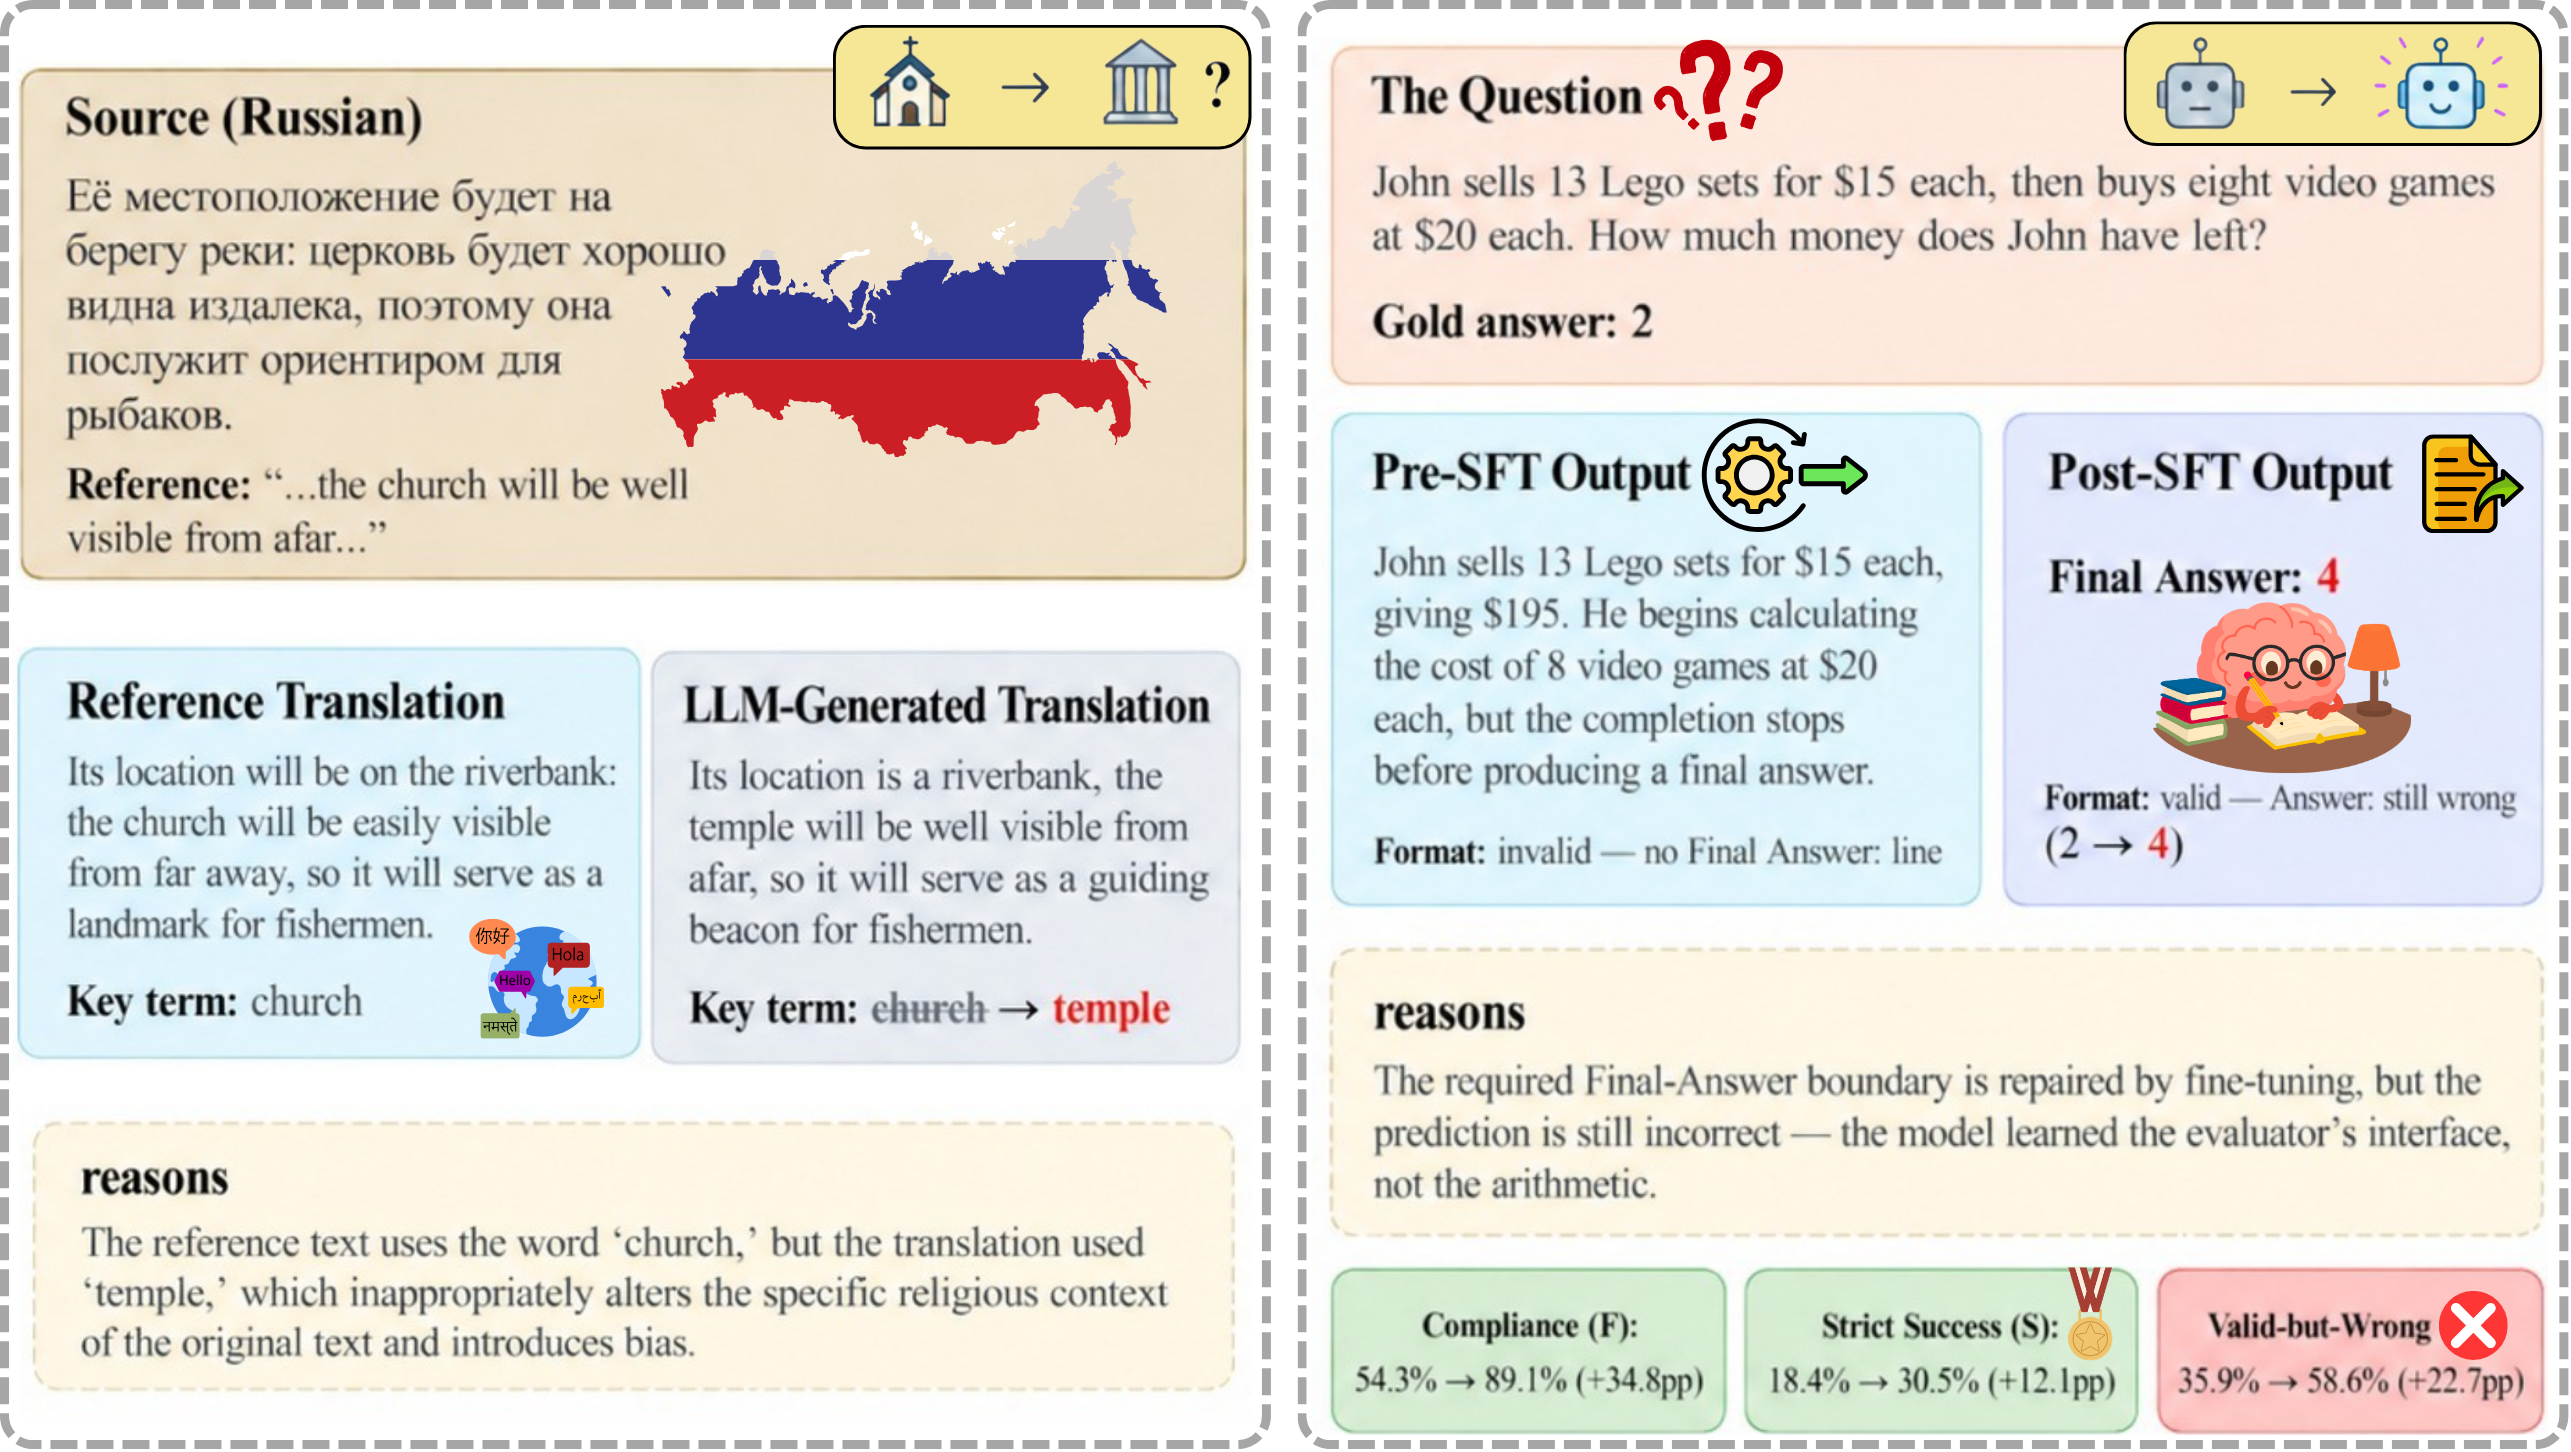
\includegraphics[width=\linewidth]{Figures/prior_work_vs_current_work.png}
    \caption{\textbf{Different evaluator blind spots can produce misleading scores.}
    \textbf{(a)} In machine translation, a meaning-changing substitution
    (\emph{church} $\rightarrow$ \emph{temple}) can remain hidden when evaluation
    emphasizes surface similarity.
    \textbf{(b)} In post-training evaluation, supervised fine-tuning repairs the
    required \texttt{Final Answer:} boundary for a GSM8K response, making it
    compliant even though its predicted answer is incorrect. CCD exposes this
    divergence by reporting compliance ($F$), strict success ($S$), and the
    valid-but-wrong rate ($F-S$) separately.}
    \label{fig:prior_work_vs_current_work}
\end{figure}


\begin{figure*}[t]
    \centering
    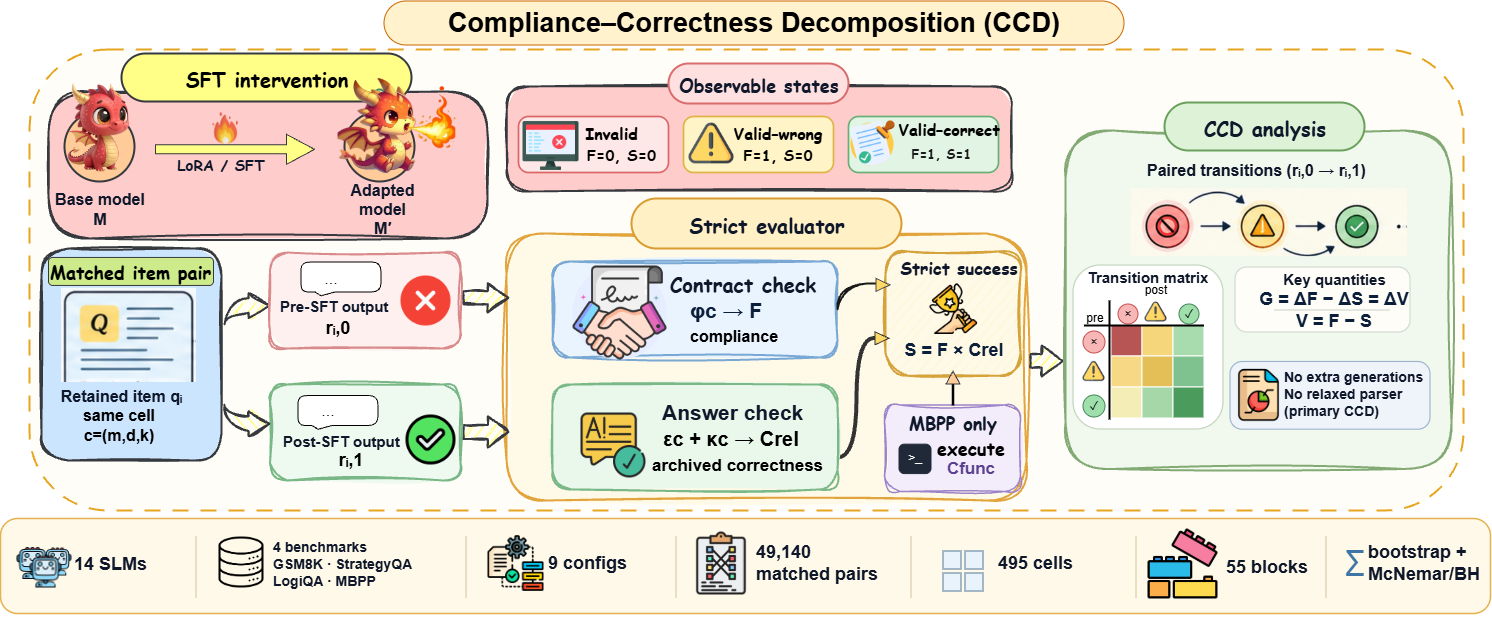
\includegraphics[width=\textwidth]{Figures/CCD.drawio.png}
    \caption{\textbf{Overview of the Compliance--Correctness Decomposition (CCD).}
    A base model and its SFT-adapted counterpart are evaluated on matched items
    within the same model--task--inference cell $c=(m,d,k)$. For each pre- and
    post-SFT response, the retained evaluator records compliance $F$ and
    parser-derived correctness $C^{\mathrm{rel}}$, with strict success defined
    as $S=F C^{\mathrm{rel}}$. These outcomes produce three observable states:
    invalid, valid but wrong, and valid and correct. CCD accounts for paired
    transitions between these states and computes the exact compliance--success
    gap $G=\Delta F-\Delta S=\Delta(F-S)$. Execution-based correctness
    $C^{\mathrm{func}}$ is evaluated separately on MBPP. The audit covers
    49,140 matched response pairs across 14 small language models, four
    benchmarks, nine inference configurations, 495 evaluation cells, and
    55 model--task blocks.}
    \label{fig:ccd_overview}
\end{figure*}



\vspace{-2mm}
\section{Methodology}
\vspace{-2mm}
We introduce the Compliance--Correctness Decomposition (CCD) as a post-hoc audit of evaluator outcomes before and after supervised fine-tuning (SFT). Rather than attributing score changes to a particular internal mechanism, we ask how the observed outcomes change under the same evaluation procedure. We separate each response into compliance with the evaluator's output contract and strict success under the original correctness check, then compare these outcomes for the same items before and after SFT. We keep parser-derived and execution-based measures separate and use them only as secondary correctness instruments.

\vspace{-2mm}
\subsection{Supervised Fine-Tuning and Paired Generation}
\label{sec:sft_paired}
\vspace{-1mm}

\noindent\textbf{Post-training intervention.}
We adapt four-bit-loaded language models with low-rank adapters \citep{dettmers2023qlora}. Training examples follow each model's chat template and use the same ``Final Answer:'' convention as evaluation. We optimize the mean assistant-token negative log likelihood:
\setcounter{equation}{1}
\begin{equation}
\mathcal{L}_{\mathrm{SFT}}(\alpha)
=-{
\sum_{z\in\mathcal{B}}
\sum_{j\in A(z)}
\log p_{\theta_0,\alpha}(z_j\mid z_{<j})
}
\mathbin{/}
{
\sum_{z\in\mathcal{B}} |A(z)|
},
\label{eq:sft_loss}
\end{equation}
where \(\theta_0\) is frozen and \(\alpha\) are trainable adapter parameters. Prompt and padding tokens are excluded. We use rank 16 adapters in attention and feed-forward projections; the recoverable run settings are reported in Appendix~\ref{app:audit}. Since targets follow the evaluation convention, SFT can affect both answers and compliance, which CCD measures separately.
\\
\noindent\textbf{Matched evaluation.}
Each cell \(c=(m,d,k)\) specifies a model, task, and inference configuration. For each retained item \(i\), we compare pre-SFT \(r_{i,0}\) and post-SFT \(r_{i,1}\) responses under identical prompts, demonstrations, decoding rules, and generation budgets. Only items observed at both stages are retained. Direct, reasoning, and few-shot settings use greedy decoding; self-consistency uses sampled completions and the original harness aggregation. We retain its recorded compliance outcome without redefining the evaluator.

\vspace{-2mm}
\subsection{Separating Compliance from Strict Success}
\label{sec:strict_definition}
\vspace{-1mm}
For each evaluation cell \(c\), the evaluator first checks whether a response follows the required output contract, extracts an answer, and then evaluates that answer against the reference. Let \(\phi_c\), \(\epsilon_c\), and \(\kappa_c\) denote these three operations. For response \(r_{i,t}\) and reference \(y_i\), we define
\begin{equation}
F_{i,t} = \phi_c(r_{i,t}), \quad
C^{\mathrm{rel}}_{i,t}
= \kappa_c\!\left(\epsilon_c(r_{i,t}),y_i\right), \quad
S_{i,t} = F_{i,t}C^{\mathrm{rel}}_{i,t}.
\label{eq:identity}
\end{equation}
Here, \(F\) is \textbf{compliance} with the implemented output contract, \(C^{\mathrm{rel}}\) is correctness under the archived parser and comparison rule, and \(S\) is \textbf{strict success}. Thus, strict success requires both a compliant response and a correct extracted answer.
\\
Our primary analysis uses the recorded values of \(F\) and \(S\) without changing the evaluator. In particular, a response that fails the contract is not reclassified as correct simply because a fallback parser can recover an answer. Parser-derived correctness and execution-based correctness are instead treated as separate secondary measures. The output contracts are summarized in Table~\ref{tab:output_contracts}, and the exact extraction and normalization rules are given in Appendix~\ref{app:instrument_full}.




\vspace{-2mm}
\subsection{Decomposing Post-Training Change}
\label{sec:decomposition}
\vspace{-1mm}
Because \(S_{i,t}\leq F_{i,t}\), every response belongs to one of three evaluator states:
\begin{equation}
Z_1=(0,0)\ \text{invalid}, \qquad
Z_2=(1,0)\ \text{valid but wrong}, \qquad
Z_3=(1,1)\ \text{valid and correct}.
\label{eq:zstates}
\end{equation}
The labels \emph{wrong} and \emph{correct} refer only to the strict evaluator's verdict.

For \(X\in\{F,S\}\), let
$\bar X_{c,t}=\frac{1}{n_c}\sum_{i\in\mathcal{I}_c}X_{i,t},
\qquad
\Delta X_c=\bar X_{c,1}-\bar X_{c,0},
\qquad
n_c=|\mathcal{I}_c|$.
The rate of valid-but-wrong responses is
$V_{c,t}=\bar F_{c,t}-\bar S_{c,t},$
since \(F-S=1\) exactly for state \(Z_2\). Therefore,
\begin{equation}
G_c\equiv\Delta F_c-\Delta S_c=\Delta V_c.
\label{eq:gap}
\end{equation}
This identity holds for every evaluation cell. We refer to this quantity as the \textbf{compliance--success gap}. It measures the change in responses that satisfy the output contract but do not receive strict correctness credit.

The gap also has a simple transition interpretation. Let \(N^{(c)}_{ab}\) denote the number of items moving from \(Z_a\) before SFT to \(Z_b\) after SFT. Then
\begin{equation} 
n_cG_c = \underbrace{N^{(c)}_{12}-N^{(c)}_{21}}_{\text{net compliance gains without credit}} + \underbrace{N^{(c)}_{32}-N^{(c)}_{23}}_{\text{net credit losses among compliant outputs}}. 
\label{eq:gap_flow}
\end{equation}

The first term captures responses that become compliant without becoming correct, while the second captures correct responses that lose strict credit while remaining compliant. Transitions from \(Z_1\) directly to \(Z_3\) improve compliance and strict success equally and therefore do not contribute to the gap.
Equations~\eqref{eq:gap} and~\eqref{eq:gap_flow} are identities over the recorded evaluator outcomes. They describe where the observed score change occurs without attributing it to a particular internal mechanism or to latent reasoning ability.

\vspace{-2mm}
\subsection{Additional Correctness Measures and Paired Transitions}
\label{sec:instruments}
\vspace{-1mm}
The three state decomposition does not assign correctness to invalid responses. To study correctness in more detail, we therefore use two additional measures. These measures provide useful information but require extra assumptions, so they remain secondary to the strict state analysis.

\noindent\textbf{Parser-derived correctness.}
The archived measure $C^{\mathrm{rel}}$ applies the evaluator's fallback extraction rules to noncompliant responses. This can show whether an answer can still be recovered when the required output format is not followed. However, its interpretation depends on the extractor. A number, option label, or code block recovered from a malformed response may not represent the model's intended answer. In addition, parser-derived labels for noncompliant natural-language responses have not been validated against human judgments. The main results in Section~\ref{sec:headline} do not depend on these labels.

\begin{equation}
C^{\mathrm{func}}_{i,t}
=
\mathbb{1}
\!\left[
\begin{gathered}
\text{the extracted program from }r_{i,t}\\
\text{passes every test in }T_i
\end{gathered}
\right].
\label{eq:functional}
\end{equation}

All selected outputs remain in the denominator. Empty or malformed programs, execution errors, timeouts, and failed tests receive zero. We compute $C^{\mathrm{func}}$ independently of compliance. Because the retained evaluators use different correctness procedures, including normalized source comparison and program execution, the archived $C^{\mathrm{rel}}$ labels are not uniformly functional judgments. We therefore use $C^{\mathrm{func}}$, rather than $C^{\mathrm{rel}}$, for claims about program behavior. In general, $FC^{\mathrm{func}}$ need not equal the archived strict success indicator $S$.

\noindent\textbf{Four-state transition accounting.}
For either secondary correctness measure $C\in\{C^{\mathrm{rel}},C^{\mathrm{func}}\}$, the pair $(C,F)$ defines four states:
$
E_1=(0,0),\qquad
E_2=(0,1),\qquad
E_3=(1,0),\qquad
E_4=(1,1).
$
A \(4\times4\) transition matrix records movement between these states for every matched item. Pure compliance gains change \(F\) from 0 to 1 while holding \(C\) fixed (\(E_1\!\rightarrow\!E_2\) or \(E_3\!\rightarrow\!E_4\)); pure correctness gains change \(C\) from 0 to 1 while holding \(F\) fixed (\(E_1\!\rightarrow\!E_3\) or \(E_2\!\rightarrow\!E_4\)). Joint changes, losses, and movements in opposing directions are retained rather than collapsed.

\noindent\textbf{Joint Success and Interaction.}
Let $J_C=FC$ denote joint success under the chosen correctness measure. Suppressing item indices, we have
\begin{equation}
\Delta J_C
=F_0\Delta C+C_0\Delta F+\Delta C\Delta F.
\label{eq:transition_identity}
\end{equation}
This identity makes the interaction between compliance and correctness explicit. Improving compliance alone increases joint success only when the item already receives correctness credit. When $C=C^{\mathrm{rel}}$, $J_C=S$ by Equation~\eqref{eq:identity}, and merging $E_1$ with $E_3$ recovers the invalid strict state $Z_1$.

\noindent\textbf{Sensitivity to fallback extraction.}
We also bound the effect of assigning correctness credit to invalid responses. For any fallback extractor that agrees with the strict evaluator on compliant outputs, write
$
C^{\mathrm{rel}}=S+R,
\qquad
R=\mathbb{1}[F=0,\ C^{\mathrm{rel}}=1].
$
Since \(0\leq\bar R_{c,t}\leq1-\bar F_{c,t}\),
\begin{equation}
\Delta C^{\mathrm{rel}}_c
\leq
\Delta S_c+1-\bar F_{c,1}
\quad\Longrightarrow\quad
D^{\mathrm{rel}}_c
\geq
G_c-\left(1-\bar F_{c,1}\right),
\label{eq:leniency}
\end{equation}
where \(D^{\mathrm{rel}}_c=\Delta F_c-\Delta C^{\mathrm{rel}}_c\). The same bound holds under common nonnegative aggregation weights. This gives a conservative bound on how much fallback credit can affect the parser-derived contrast without assuming that the recovered labels are correct.

\vspace{-2mm}
\subsection{Aggregation, Uncertainty, and Robustness}
\label{sec:aggregation}
\vspace{-1mm}
CCD computes changes within cells before aggregation. For \(X\in\{F,S,V,C^{\mathrm{rel}},C^{\mathrm{func}}\}\), we give each eligible cell equal weight:
\begin{equation}
\Delta X=
\frac{1}{|\mathcal{C}_X|}
\sum_{c\in\mathcal{C}_X}\Delta X_c,
\qquad
G=\Delta F-\Delta S,
\qquad
D^{\mathrm{rel}}=\Delta F-\Delta C^{\mathrm{rel}}.
\label{eq:aggregation}
\end{equation}
Here, \(\mathcal{C}_X\) contains cells where \(X\) is observed, with common cells and weights used for each contrast. Functional correctness uses the common execution-eligible subset. Equal-cell weighting prevents larger cells from dominating. We also report observation-weighted and equal-model estimates. Pooled transition counts directly describe item pairs and recover the observation-weighted gap.
\\
\noindent\textbf{Uncertainty.}
Inference configurations are repeated evaluations within model-task blocks, not independent units. We therefore use 10,000 hierarchical bootstrap replicates (seed 42), sampling models and their task blocks with replacement while retaining all configurations within each block. The 2.5th and 97.5th percentiles give 95\% intervals. These quantify variation across the observed evaluation hierarchy, not training seeds; blocks sharing an adapter likewise do not show independent SFT runs.
\\
\noindent\textbf{Paired significance tests.}
We use exact McNemar tests for discordant paired outcomes within each cell \citep{mcnemar1947note}, with Benjamini--Hochberg correction across cells for each outcome (\(q<.05\)) \citep{benjamini1995controlling}. Because cells may share models, tasks, or adapters, these tests are local diagnostics, not independent replications or aggregate inference.
\\
\noindent\textbf{Robustness.}
We vary aggregation weights, omit each model or task in turn, separate greedy and sampled decoding, and replace parser-derived with execution-based correctness where available. All statistics use retained paired records and require no additional generations.

\vspace{-2mm}
\section{Experiments}
\vspace{-2mm}
\noindent\textbf{Models and benchmarks.}
We evaluate 14 instruction-tuned language models ranging from 270M to 8B parameters across four benchmarks: GSM8K, LogiQA, MBPP, and StrategyQA. These benchmarks cover numerical reasoning, multiple-choice reasoning, program synthesis, and Boolean reasoning, respectively, with different output contracts and correctness criteria. All models are evaluated before and after SFT using the same prompts, item sets, inference configurations, and evaluator versions within each comparison.
\\
\noindent\textbf{Inference configurations.}
For each model and benchmark, we consider nine inference configurations covering zero-shot, chain-of-thought, few-shot, and self-consistency settings. We retain only item-level matches observed at both stages, giving 49,140 paired responses across 495 evaluation cells and 55 model-task blocks. This paired design ensures that changes in compliance and strict success are measured on the same items rather than on potentially different samples.
\\
\noindent\textbf{Evaluation protocol.}
The primary analysis uses the evaluator's original output contract and correctness procedure. We preserve historical evaluator differences rather than modifying them to create a common definition after the fact. We additionally evaluate MBPP programs against a standardized execution-based test suite to provide a common functional correctness measure across historical evaluator versions.
\\
\noindent\textbf{Implementation and provenance.}
Detailed model configurations, item selection, evaluator rules, SFT settings, provenance checks, and the standardized MBPP evaluation protocol are provided in Appendix~\ref{app:Evaluation-Design}. All primary analyses are computed from the retained paired records and require no additional model generations.


\begin{figure}[t]
\centering
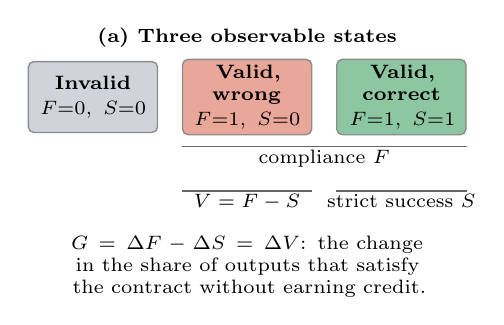
\begin{tikzpicture}[font=\scriptsize, baseline=(current bounding box.center),
  box/.style={draw=black!45, line width=0.5pt, rounded corners=2pt,
    minimum height=0.9cm, text width=1.5cm, align=center, inner sep=2pt}]
  \node[box, fill=ccdinvalid] (z1) at (0,0) {\textbf{Invalid}\\[1pt]$F{=}0,\ S{=}0$};
  \node[box, fill=ccdwrong, right=0.3cm of z1] (z2) {\textbf{Valid, wrong}\\[1pt]$F{=}1,\ S{=}0$};
  \node[box, fill=ccdcorrect, right=0.3cm of z2] (z3) {\textbf{Valid, correct}\\[1pt]$F{=}1,\ S{=}1$};
  \coordinate (m23) at ($(z2.south)!0.5!(z3.south)$);
  \draw[black!60, line width=0.6pt] ([yshift=-4pt]z2.south west) -- ([yshift=-4pt]z3.south east);
  \node[below=5pt of m23, inner sep=0pt] {compliance $F$};
  \draw[black!60, line width=0.6pt] ([yshift=-20pt]z3.south west) -- ([yshift=-20pt]z3.south east);
  \node[below=21pt of z3.south, inner sep=0pt] {strict success $S$};
  \draw[black!60, line width=0.6pt] ([yshift=-20pt]z2.south west) -- ([yshift=-20pt]z2.south east);
  \node[below=21pt of z2.south, inner sep=0pt] {$\VW=F-S$};
  \node[above=4pt of z2.north, inner sep=0pt, font=\scriptsize\bfseries] {(a) Three observable states};
  \node[below=36pt of z2.south, inner sep=0pt, text width=5.2cm, align=center]
    {$\Gap=\Delta F-\Delta S=\Delta\VW$: the change in the share of outputs that satisfy the contract without earning credit.};
\end{tikzpicture}
\hfill
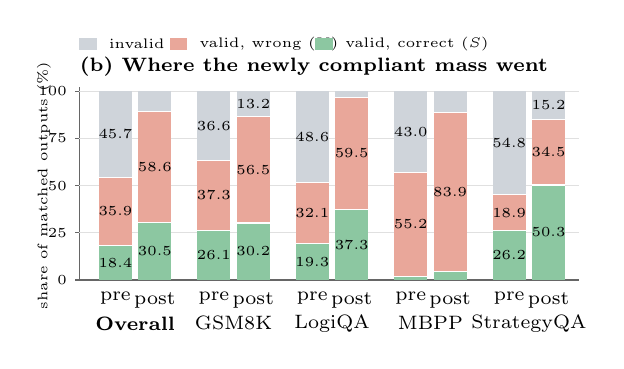
\begin{tikzpicture}[font=\scriptsize, baseline=(current bounding box.center)]
  % axis
  \draw[black!60] (0,0) -- (0,2.45);
  \foreach \y/\lab in {0/0,0.6/25,1.2/50,1.8/75,2.4/100}{
    \draw[black!60] (-0.05,\y) -- (0,\y);
    \node[left=1pt, font=\tiny] at (0,\y) {\lab};
    \draw[black!12, line width=0.3pt] (0,\y) -- (6.35,\y);
  }
  \node[rotate=90, font=\tiny] at (-0.45,1.2) {share of matched outputs (\%)};
  \draw[black!60] (0,0) -- (6.35,0);
  % bars: x, invalid, valid-but-wrong, valid-and-correct, label
  \ccdbar{0.25}{45.7}{35.9}{18.4}{pre}
  \ccdbar{0.75}{10.9}{58.6}{30.5}{post}
  \ccdbar{1.50}{36.6}{37.3}{26.1}{pre}
  \ccdbar{2.00}{13.2}{56.5}{30.2}{post}
  \ccdbar{2.75}{48.6}{32.1}{19.3}{pre}
  \ccdbar{3.25}{3.2}{59.5}{37.3}{post}
  \ccdbar{4.00}{43.0}{55.2}{1.8}{pre}
  \ccdbar{4.50}{11.5}{83.9}{4.6}{post}
  \ccdbar{5.25}{54.8}{18.9}{26.2}{pre}
  \ccdbar{5.75}{15.2}{34.5}{50.3}{post}
  % group labels
  \node[font=\scriptsize\bfseries] at (0.71,-0.55) {Overall};
  \node[font=\scriptsize] at (1.96,-0.55) {GSM8K};
  \node[font=\scriptsize] at (3.21,-0.55) {LogiQA};
  \node[font=\scriptsize] at (4.46,-0.55) {MBPP};
  \node[font=\scriptsize] at (5.71,-0.55) {StrategyQA};
  % legend
  \node[anchor=south west, inner sep=0pt, font=\scriptsize\bfseries] at (0,2.58) {(b) Where the newly compliant mass went};
  \fill[ccdinvalid] (0,2.92) rectangle ++(0.22,0.16); \node[right=1pt, font=\tiny] at (0.22,3.0) {invalid};
  \fill[ccdwrong] (1.15,2.92) rectangle ++(0.22,0.16); \node[right=1pt, font=\tiny] at (1.37,3.0) {valid, wrong ($\VW$)};
  \fill[ccdcorrect] (3.0,2.92) rectangle ++(0.22,0.16); \node[right=1pt, font=\tiny] at (3.22,3.0) {valid, correct ($S$)};
\end{tikzpicture}
\caption{\textbf{The Compliance--Correctness Decomposition.} (a)~Strict
success $S$ implies compliance $F$, so every output is invalid, valid but
wrong, or valid and correct, and the valid-but-wrong rate $\VW=F-S$ is
observable without any relaxed parsing. (b)~Equal-cell shares of the three
states before and after SFT, pooled over 495 cells and by benchmark. SFT
converts most invalid outputs into compliant ones, but the majority of the
newly compliant mass lands in the valid-but-wrong state: pooled $\VW$ grows
from 35.9\% to 58.6\%.}
\label{fig:overview}
\end{figure}

\vspace{-3mm}
\section{Experimental Findings}
\label{sec:results}
\vspace{-3mm}
\subsection{Overall Findings}
\label{sec:headline}
\vspace{-2mm}
\textbf{SFT improves compliance more than correctness.}
Table~\ref{tab:headline} reports the primary equal-cell estimates, with
Figure~\ref{fig:overview}(b) visualizing the changes. SFT increases strict
success from 18.35\% to 30.47\% ($+12.12$\pp{}; 95\% CI
$[8.08,16.56]$), while compliance rises from 54.28\% to 89.06\%
($+34.78$\pp{}; CI $[23.29,47.82]$). The valid-but-wrong rate consequently
increases by 22.66\pp{} ($[13.42,33.66]$), closing 76.1\% of compliance
headroom but only 14.8\% of strict-success headroom.
The pattern holds across all benchmarks, with the gap ranging from
$+15.59$\pp{} on StrategyQA to $+28.72$\pp{} on MBPP. On MBPP, compliance
gains 31.48\pp{} while archived strict success changes little. Thus, greater
compliance does not necessarily translate into greater task success.
Cell-level paired tests provide similar evidence (Table~\ref{tab:significance}
in Appendix~\ref{app:significance}). After FDR correction, compliance changes
significantly in 290 of 495 cells (274 increases, 16 decreases), compared with
183 for strict success (176 increases, 7 decreases). Parser-derived
correctness changes significantly in only 67 cells
(Appendix~\ref{app:significance}). Overall, strict scores substantially
understate changes in evaluator-facing behavior, while the decomposition itself
requires no relaxed parser.
\\
\noindent\textbf{Most gains are compliance without correctness.}
Equation~\eqref{eq:gap_flow} identifies where the gap comes from, and
Table~\ref{tab:strict_matrix} shows this directly without any extractor.
Of 22{,}418 outputs that were invalid before SFT, 17{,}641 become compliant,
but 11{,}843 (67.1\%) remain wrong. After accounting for reverse moves, this
flow contributes 11{,}424 items (23.25\pp{}) to the gap. In contrast, compliant
wrong answers gain only 291 net correct transitions ($-0.59$\pp{}), while
189 correct outputs lose compliance. Together these flows give
$(11{,}424-291)/49{,}140=22.66$\pp{}, exactly matching the observation-weighted
gap. Thus, the large compliance gain is driven primarily by outputs becoming
valid without becoming correct.
\\
\noindent\textbf{The pattern persists under relaxed extraction.}
The four-state analysis in Figure~\ref{fig:transition} further separates
invalid responses by parser-derived correctness. Half of all pairs (50.61\%)
remain in the same state, while the largest transition is
$\Eone\!\to\!\Etwo$ (9{,}924 pairs, 20.2\%), where SFT fixes the output format
without fixing the answer. Pure compliance gains account for 24.88\% of all
pairs, compared with 6.37\% pure correctness gains and 7.11\% joint gains.
Parser-derived correctness increases by only 3.57\pp{} (CI
$[0.85,6.65]$), despite the 34.78\pp{} compliance gain, giving
$\Drel=31.22$\pp{} (CI $[19.47,44.17]$). The relaxed analysis therefore
reinforces the strict result, while the main conclusion remains independent
of parser-derived labels for invalid outputs.

\begin{table}[t]
\centering
\small
\setlength{\tabcolsep}{4pt}
\caption{\textbf{Primary equal-cell levels before and after SFT (\%) and the
compliance--success gap $\Gap=\Delta F-\Delta S=\Delta\VW$ (pp; overall 95\%
CI $[13.42,33.66]$).} On MBPP the archived strict flag inherits the original
harness's limited execution coverage (Section~\ref{sec:mbpp_design});
standardized re-execution results are in Section~\ref{sec:mbpp}.
Green shading (\ccdlegend{}) highlights larger compliance--success gaps $\Gap$. Color denotes gap size, not better performance.}
\label{tab:headline}
\begin{tabular*}{\linewidth}{@{\extracolsep{\fill}}lrrrrrrrr@{}}
\toprule
& & \multicolumn{2}{c}{\textbf{Compliance $F$}}
  & \multicolumn{2}{c}{\textbf{Strict success $S$}}
  & \multicolumn{2}{c}{\textbf{Valid but wrong $\VW$}}
  & \\
\cmidrule(lr){3-4}\cmidrule(lr){5-6}\cmidrule(lr){7-8}
\textbf{Benchmark} & \textbf{Cells} & \textbf{Pre} & \textbf{Post} & \textbf{Pre} & \textbf{Post} & \textbf{Pre} & \textbf{Post} & $\boldsymbol{\Gap}$ \\
\midrule
GSM8K      & 126 & 63.39 & 86.78 & 26.10 & 30.24 & 37.30 & 56.53 & \ccdheat{24}$+19.24$\\
LogiQA     & 117 & 51.38 & 96.76 & 19.33 & 37.26 & 32.05 & 59.50 & \ccdheat{59}$+27.45$\\
MBPP       & 126 & 56.97 & 88.45 &  1.81 &  4.57 & 55.16 & 83.88 & \ccdheat{65}$+28.72$\\
StrategyQA & 126 & 45.17 & 84.82 & 26.24 & 50.31 & 18.93 & 34.51 & \ccdheat{8}$+15.59$\\
\midrule
\textbf{Overall} & \textbf{495} & \textbf{54.28} & \textbf{89.06} & \textbf{18.35} & \textbf{30.47} & \textbf{35.93} & \textbf{58.59} & \ccdheat{39}$\boldsymbol{+22.66}$\\
\bottomrule
\end{tabular*}
\end{table}


\begin{table}[t]
\centering
\small
\setlength{\tabcolsep}{6pt}
\caption{\textbf{Pooled strict-state transition matrix over 49{,}140 matched outputs
(count and share of all pairs).} States use only $F$ and $S$
(Eq.~\ref{eq:zstates}), so no relaxed extraction is involved. By
Eq.~\eqref{eq:gap_flow}, the gap is $(N_{12}-N_{21})+(N_{32}-N_{23})
=(11{,}843-419)+(2{,}586-2{,}877)=11{,}133$ items, i.e.\ 22.66\pp{}.
Green shading (\ccdlegend{}) highlights larger counts in the valid-but-wrong destination column.}
\label{tab:strict_matrix}
\begin{tabular}{lrrrr}
\toprule
& \multicolumn{3}{c}{\textbf{Post-SFT strict state}} & \\
\cmidrule(lr){2-4}
\textbf{Pre-SFT strict state} & $Z_1$ invalid & $Z_2$ valid, wrong & $Z_3$ valid, correct & \textbf{Total}\\
\midrule
$Z_1$ invalid        & 4,777 (9.7\%)  & \ccdheat{53}\textbf{11,843 (24.1\%)} & 5,798 (11.8\%) & 22,418\\
$Z_2$ valid, wrong   & 419 (0.9\%)    & \ccdheat{65}14,431 (29.4\%)          & 2,877 (5.9\%)  & 17,727\\
$Z_3$ valid, correct & 189 (0.4\%)    & \ccdheat{8}2,586 (5.3\%)            & 6,220 (12.7\%) & 8,995\\
\midrule
\textbf{Total}       & 5,385          & 28,860                   & 14,895         & 49,140\\
\bottomrule
\end{tabular}
\vspace{-2mm}
\end{table}

% \begin{figure}[t]
% \centering
% \begin{tikzpicture}[
%   cell/.style={draw=white, line width=0.7pt, minimum width=1.4cm,
%     minimum height=0.55cm, align=center, inner sep=1pt},
%   every node/.style={font=\scriptsize}]
%   \matrix (m) [matrix of nodes, nodes={cell}, row sep=1pt, column sep=1pt] {
%     |[fill=ccdgray]|   \shortstack{3,228\\6.6\%} &
%     |[fill=ccdblue]|   \shortstack{\textbf{9,924}\\\textbf{20.2\%}} &
%     |[fill=ccdgreen]|  \shortstack{251\\0.5\%} &
%     |[fill=ccdpurple]| \shortstack{3,494\\7.1\%} \\
%     |[fill=ccdred]|    \shortstack{368\\0.7\%} &
%     |[fill=ccdgray]|   \shortstack{14,431\\29.4\%} &
%     |[fill=ccdred]|    \shortstack{51\\0.1\%} &
%     |[fill=ccdgreen]|  \shortstack{2,877\\5.9\%} \\
%     |[fill=ccdred]|    \shortstack{308\\0.6\%} &
%     |[fill=ccdred]|    \shortstack{1,919\\3.9\%} &
%     |[fill=ccdgray]|   \shortstack{990\\2.0\%} &
%     |[fill=ccdblue]|   \shortstack{2,304\\4.7\%} \\
%     |[fill=ccdred]|    \shortstack{111\\0.2\%} &
%     |[fill=ccdred]|    \shortstack{2,586\\5.3\%} &
%     |[fill=ccdred]|    \shortstack{78\\0.2\%} &
%     |[fill=ccdgray]|   \shortstack{6,220\\12.7\%} \\
%   };
%   \foreach \j/\lab in {1/{$\Eone$ wrong, invalid},2/{$\Etwo$ wrong, valid},3/{$\Ethree$ correct, invalid},4/{$\Efour$ correct, valid}}
%     \node[above=2pt of m-1-\j.north, align=center, text width=1.4cm] {\lab};
%   \foreach \i/\lab in {1/$\Eone$,2/$\Etwo$,3/$\Ethree$,4/$\Efour$}
%     \node[left=3pt of m-\i-1.west] {\lab};
%   \node[font=\scriptsize\bfseries, anchor=south] at ([yshift=24pt]m.north) {Post-SFT state};
%   \node[font=\scriptsize\bfseries, rotate=90] at ([xshift=-26pt]m.west) {Pre-SFT state};
%   \node[anchor=north, inner sep=0pt, font=\tiny] at ([yshift=-6pt]m.south) {%
%     \raisebox{-0.2ex}{\textcolor{ccdblue}{\rule{8pt}{6pt}}}\hspace{2pt}pure compliance gain\hspace{7pt}%
%     \raisebox{-0.2ex}{\textcolor{ccdgreen}{\rule{8pt}{6pt}}}\hspace{2pt}pure correctness gain\hspace{7pt}%
%     \raisebox{-0.2ex}{\textcolor{ccdpurple}{\rule{8pt}{6pt}}}\hspace{2pt}joint gain\hspace{7pt}%
%     \raisebox{-0.2ex}{\textcolor{ccdred}{\rule{8pt}{6pt}}}\hspace{2pt}loss or trade-off\hspace{7pt}%
%     \raisebox{-0.2ex}{\textcolor{ccdgray}{\rule{8pt}{6pt}}}\hspace{2pt}unchanged};
% \end{tikzpicture}
% \caption{Pooled transition matrix over 49{,}140 matched outputs under the
% relaxed extractor; each cell reports the count and share of all pairs. Rows
% are pre-SFT states and columns post-SFT states, with coordinates (correct,
% valid). The dominant off-diagonal transition, $\Eone\!\to\!\Etwo$, becomes
% contract-valid while remaining wrong. Contract-invalid non-MBPP labels are
% parser-derived (Section~\ref{sec:instruments}).}
% \label{fig:transition}
% \end{figure}

\begin{figure}[t]
\centering
\begin{minipage}[t]{0.55\linewidth}
\centering
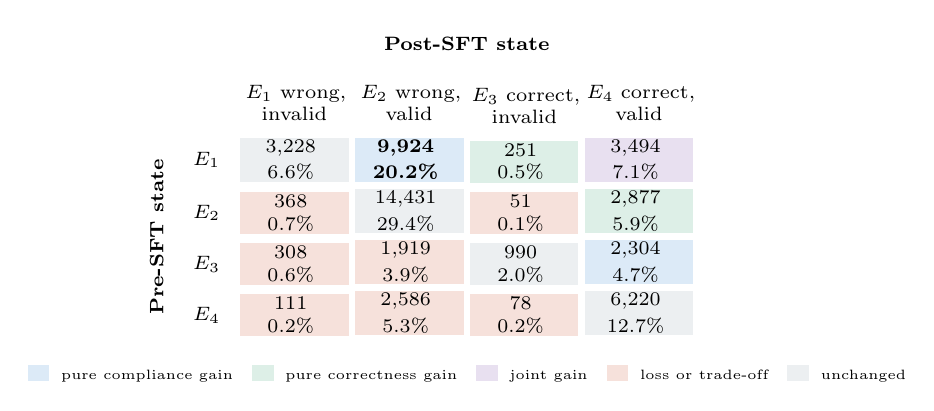
\begin{tikzpicture}[
  cell/.style={draw=white, line width=0.7pt, minimum width=1.4cm,
    minimum height=0.55cm, align=center, inner sep=1pt},
  every node/.style={font=\scriptsize}]

  \matrix (m) [matrix of nodes, nodes={cell}, row sep=1pt, column sep=1pt] {
    |[fill=ccdgray]|   \shortstack{3,228\\6.6\%} &
    |[fill=ccdblue]|   \shortstack{\textbf{9,924}\\\textbf{20.2\%}} &
    |[fill=ccdgreen]|  \shortstack{251\\0.5\%} &
    |[fill=ccdpurple]| \shortstack{3,494\\7.1\%} \\
    |[fill=ccdred]|    \shortstack{368\\0.7\%} &
    |[fill=ccdgray]|   \shortstack{14,431\\29.4\%} &
    |[fill=ccdred]|    \shortstack{51\\0.1\%} &
    |[fill=ccdgreen]|  \shortstack{2,877\\5.9\%} \\
    |[fill=ccdred]|    \shortstack{308\\0.6\%} &
    |[fill=ccdred]|    \shortstack{1,919\\3.9\%} &
    |[fill=ccdgray]|   \shortstack{990\\2.0\%} &
    |[fill=ccdblue]|   \shortstack{2,304\\4.7\%} \\
    |[fill=ccdred]|    \shortstack{111\\0.2\%} &
    |[fill=ccdred]|    \shortstack{2,586\\5.3\%} &
    |[fill=ccdred]|    \shortstack{78\\0.2\%} &
    |[fill=ccdgray]|   \shortstack{6,220\\12.7\%} \\
  };

  \foreach \j/\lab in {
    1/{$\Eone$ wrong, invalid},
    2/{$\Etwo$ wrong, valid},
    3/{$\Ethree$ correct, invalid},
    4/{$\Efour$ correct, valid}
  }
    \node[above=2pt of m-1-\j.north, align=center, text width=1.4cm] {\lab};

  \foreach \i/\lab in {
    1/$\Eone$,2/$\Etwo$,3/$\Ethree$,4/$\Efour$
  }
    \node[left=3pt of m-\i-1.west] {\lab};

  \node[font=\scriptsize\bfseries, anchor=south]
    at ([yshift=24pt]m.north) {Post-SFT state};

  \node[font=\scriptsize\bfseries, rotate=90]
    at ([xshift=-26pt]m.west) {Pre-SFT state};

  \node[anchor=north, inner sep=0pt, font=\tiny]
    at ([yshift=-6pt]m.south) {%
    \resizebox{0.92\linewidth}{!}{%
    \raisebox{-0.2ex}{\textcolor{ccdblue}{\rule{8pt}{6pt}}}
    \hspace{2pt}pure compliance gain\hspace{7pt}%
    \raisebox{-0.2ex}{\textcolor{ccdgreen}{\rule{8pt}{6pt}}}
    \hspace{2pt}pure correctness gain\hspace{7pt}%
    \raisebox{-0.2ex}{\textcolor{ccdpurple}{\rule{8pt}{6pt}}}
    \hspace{2pt}joint gain\hspace{7pt}%
    \raisebox{-0.2ex}{\textcolor{ccdred}{\rule{8pt}{6pt}}}
    \hspace{2pt}loss or trade-off\hspace{7pt}%
    \raisebox{-0.2ex}{\textcolor{ccdgray}{\rule{8pt}{6pt}}}
    \hspace{2pt}unchanged}};

\end{tikzpicture}

\captionof{figure}{\textbf{Pooled transition matrix over 49{,}140 matched outputs under the relaxed extractor.} Cells show count and share; rows are pre-SFT and columns post-SFT, with states $(\text{correct},\text{valid})$. The dominant transition, $\Eone\!\to\!\Etwo$, becomes valid while remaining wrong. Non-MBPP invalid labels are parser-derived.}
\label{fig:transition}
\end{minipage}
\hfill
\begin{minipage}[t]{0.43\linewidth}
\centering
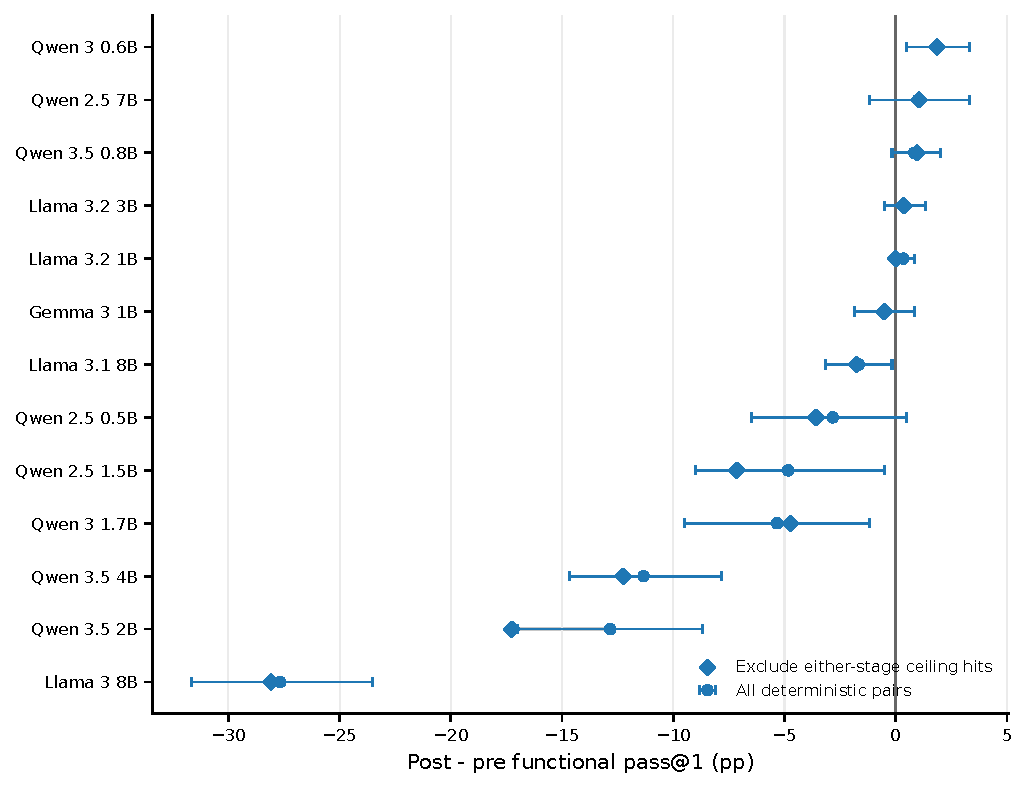
\includegraphics[width=\linewidth]{fig3_mbpp_heterogeneity.pdf}

\captionof{figure}{\textbf{Per-checkpoint change in deterministic MBPP pass@1 after SFT (pp).} Circles show all 600 pairs with paired-bootstrap 95\% intervals; diamonds exclude generation-ceiling pairs. All checkpoints starting above 15\% decline, while none starting below 5\% does.}
\label{fig:mbpp}
\end{minipage}
\end{figure}

\vspace{-3mm}
\subsection{Robustness Across Analysis Choices}
\label{sec:robust}
\vspace{-2mm}
\noindent\textbf{The gap survives analysis choices.}
Table~\ref{tab:robust_main} shows that the strict gap remains positive under
alternative weighting, decoding regimes, and model or benchmark exclusions,
ranging from 20.01 to 26.22\pp{}. Leave-one-model-out estimates range from
18.84 to 24.27\pp{}, and leave-one-benchmark-out estimates from 20.59 to
25.08\pp{} (Table~\ref{tab:lodo}). At finer granularity, the gap is positive for all 14 models,
four benchmarks, and nine inference configurations
(Tables~\ref{tab:permodel} and~\ref{tab:perconfig_main} in
Appendix~\ref{app:secondary_main_tables}). The same pattern holds for the
parser-derived contrast.
\\
\noindent\textbf{The finding does not depend on the extractor.}
The primary strict analysis uses no relaxed extraction. More generally,
Eq.~\eqref{eq:leniency} bounds the parser-derived gap at
$\Drel\ge11.72$\pp{} even under the most favorable possible treatment of
invalid outputs. The documented extractor gives $\Drel=31.22$\pp{}, while
crediting every invalid output gives 57.45\pp{}; the strict boundary gives
22.66\pp{} (Appendix~\ref{app:parser_dataset}). Thus, the qualitative
conclusion holds across substantially different treatments of invalid
responses.
\\
\noindent\textbf{The effect follows compliance headroom.}
Cells with very low initial compliance show the largest changes: the lowest
quartile starts at 0.56\% compliance, gains 71.61\pp{}, and has
$\Drel=66.63$\pp{}. At the highest quartile, starting at 99.52\%, compliance
changes by only $-0.85$\pp{} and $\Drel=-2.26$\pp{}. This shows that the
decomposition is not a scale-free effect size, but tracks the available
compliance headroom (Table~\ref{tab:headroom_main}). More broadly, compliance and parser-derived correctness
are only weakly coupled across cells (Pearson $r=.28$), with compliance
improving without a correctness gain in 149 of 495 cells (30.1\%).







\begin{table}[t]
\centering
\footnotesize

\caption{\textbf{Robustness of the compliance--success gap (pp).} Strict columns use
the evaluator's own verdict; parser-derived columns use the relaxed extractor.
The three largest MBPP decliners are Llama~3~8B, Qwen~3.5~2B, and
Qwen~3.5~4B (Section~\ref{sec:mbpp}); ranges are minima and maxima over the
omitted units.
Green shading (\ccdlegend{}) highlights larger values of the primary gap $\Gap$; other columns are unshaded.}
\label{tab:robust_main}
\setlength{\tabcolsep}{1.4pt}
\begin{tabular*}{\linewidth}{@{\extracolsep{\fill}}lrrrrrr@{}}
\toprule
& & \multicolumn{3}{c}{\textbf{Strict evaluator (primary)}} & \multicolumn{2}{c}{\textbf{Parser-derived}}\\
\cmidrule(lr){3-5}\cmidrule(lr){6-7}
\textbf{Analysis} & \textbf{Cells} & $\boldsymbol{\Delta S}$ & $\boldsymbol{\Delta F}$ & $\boldsymbol{\Gap}$ & $\boldsymbol{\Delta\Crel}$ & $\boldsymbol{\Drel}$\\
\midrule
Primary, equal-cell weighting & 495 & $+12.12$ & $+34.78$ & \ccdheat{32}$\boldsymbol{+22.66}$ & $+3.57$ & $+31.22$\\
\quad 95\% hierarchical-bootstrap CI & & $[8.08,16.56]$ & $[23.29,47.82]$ & $[13.42,33.66]$ & $[0.85,6.65]$ & $[19.47,44.17]$\\
Observation-weighted & 495 & $+12.01$ & $+34.66$ & \ccdheat{32}$+22.66$ & $+3.56$ & $+31.10$\\
Equal-model weighted & 495 & $+12.24$ & $+35.37$ & \ccdheat{37}$+23.13$ & $+3.56$ & $+31.81$\\
\addlinespace[2pt]
Excluding MBPP & 369 & $+15.32$ & $+35.91$ & \ccdheat{13}$+20.59$ & $+4.91$ & $+31.00$\\
Excluding three largest MBPP decliners & 387 & $+12.65$ & $+38.87$ & \ccdheat{65}$+26.22$ & $+2.61$ & $+36.26$\\
Excluding both & 288 & $+15.93$ & $+40.26$ & \ccdheat{48}$+24.33$ & $+3.49$ & $+36.78$\\
\addlinespace[2pt]
Deterministic configurations only & 330 & $+12.28$ & $+36.27$ & \ccdheat{45}$+23.99$ & $+3.42$ & $+32.85$\\
Self-consistency configurations only & 165 & $+11.80$ & $+31.81$ & \ccdheat{8}$+20.01$ & $+3.85$ & $+27.95$\\
\addlinespace[2pt]
Leave one model out (range) & 459--468 & $11.55$--$12.57$ & $30.39$--$36.84$ & $18.84$--$24.27$ & $2.86$--$3.96$ & $27.11$--$33.33$\\
Leave one benchmark out (range) & 369--378 & $8.04$--$15.32$ & $31.51$--$38.68$ & $20.59$--$25.08$ & $1.63$--$4.91$ & $29.56$--$34.47$\\
\bottomrule
\end{tabular*}
\vspace{-2mm}
\end{table}



\begin{table}[t]
\centering
\footnotesize
\setlength{\tabcolsep}{3pt}
\begin{tabular*}{\linewidth}{@{\extracolsep{\fill}}lrrrrr@{}}
\toprule
\multicolumn{6}{@{}l}{\textbf{A. Functional summary} (\%, changes in pp)}\\
\textbf{Scope} & \textbf{Pairs} & \textbf{Pre} & \textbf{Post} & $\boldsymbol{\Delta\Cfunc}$ \textbf{[95\% CI]} & $\boldsymbol{\Delta F}$\\
\midrule
All nine configurations (selected-output accuracy) & 11,700 & 18.99 & 15.33 & \ccdheat{65}$-3.66$ $[-7.71,-0.50]$ & $+27.21$\\
Six deterministic configurations (pass@1) & 7,800 & 19.62 & 14.79 & \ccdheat{28}$-4.82$ $[-9.65,-1.05]$ & $+26.31$\\
Deterministic, either-stage ceiling hits removed & 6,436 & 21.73 & 16.26 & \ccdheat{8}$-5.47$ $[-10.57,-1.30]$ & --\\
\midrule
\multicolumn{6}{@{}l}{\textbf{B. Paired pass/failure accounting} (all 11,700 pairs)}\\
\textbf{Failure class} & \multicolumn{2}{c}{\textbf{Pass$\to$fail}} & \multicolumn{2}{c}{\textbf{Fail$\to$pass}} & \textbf{Net loss}\\
\midrule
Assertion failure   & \multicolumn{2}{c}{525} & \multicolumn{2}{c}{265} & \ccdheat{65}$+260$\\
Syntax error        & \multicolumn{2}{c}{189} & \multicolumn{2}{c}{49}  & \ccdheat{43}$+140$\\
TypeError           & \multicolumn{2}{c}{97}  & \multicolumn{2}{c}{73}  & \ccdheat{21}$+24$\\
IndexError          & \multicolumn{2}{c}{24}  & \multicolumn{2}{c}{6}   & \ccdheat{20}$+18$\\
AttributeError      & \multicolumn{2}{c}{16}  & \multicolumn{2}{c}{0}   & \ccdheat{20}$+16$\\
NameError           & \multicolumn{2}{c}{105} & \multicolumn{2}{c}{152} & \ccdheat{8}$-47$\\
All classes         & \multicolumn{2}{c}{1,014} & \multicolumn{2}{c}{586} & $+428$\\
\bottomrule
\end{tabular*}
\caption{\textbf{Execution-based MBPP results for the 13 checkpoints with
standardized test mappings.} Panel~A intervals are model-cluster bootstrap
CIs; the third row removes every deterministic pair whose generation reached
the model's token ceiling at either stage. Panel~B lists the failure classes
with the largest paired imbalances; net counts are accounting quantities, not
causal attributions.
Only functional change in A and net loss in B are shaded. Green (\ccdlegend{}) encodes larger signed values within each panel, not statistical significance.}
\label{tab:mbpp_main}
\end{table}


\vspace{-3mm}
\subsection{MBPP: Compliance Rises While Functional Correctness Falls}
\label{sec:mbpp}
\vspace{-2mm}
MBPP provides an independent correctness check because generated programs can
be executed. Across all nine configurations, selected-output functional
accuracy falls from 18.99\% to 15.33\% ($-3.66$\pp{}; model-cluster CI
$[-7.71,-0.50]$), while compliance rises by 27.21\pp{}. Across the six
deterministic configurations, pass@1 falls from 19.62% to 14.79%
($-4.82$\pp{}; CI $[-9.65,-1.05]$) against a 26.31\pp{} compliance gain.
The compliance--function gap is positive in every configuration, and 64 of
117 cells (54.7\%) improve in compliance without improving functional
correctness (Appendix~\ref{app:mbpp_config}).
Configuration-level and checkpoint-level results are reported in
Tables~\ref{tab:mbpp_config_func} and~\ref{tab:mbpp_model_all9}, respectively.
\\
\noindent\textbf{Where functional correctness is lost.}
Of 2{,}222 pre-SFT passes, 1{,}014 become failures, while 586 failures become
passes, giving a net loss of 428 passes (Table~\ref{tab:mbpp_main}B).
Assertion failures account for 260 of this loss (60.7\%) and syntax errors for
140 (32.7\%). Undefined-name errors instead decline by 47, suggesting that
post-SFT programs become more self-contained without becoming more correct.
Marginal execution outcomes are reported in Table~\ref{tab:mbpp_status_counts}.
The qualitative examples in Appendix~\ref{app:qualitative} show the same
pattern: an initially passing program is replaced by one that better follows
the output contract but fails execution.
\\
\noindent\textbf{The decline is not explained by evaluation artifacts.}
Every non-executable program remains a failure in the denominator, so malformed
outputs are not discarded. Truncation also cannot explain the result: generation
ceiling hits fall from 16.68\% to 1.14\%, and excluding every pair that hits
the ceiling at either stage leaves 6{,}436 pairs with a larger decline of
$-5.47$\pp{} (CI $[-10.57,-1.30]$).
\\
\noindent\textbf{The effect is heterogeneous.}
Figure~\ref{fig:mbpp} visualizes this heterogeneity; the plotted values are
listed in Table~\ref{tab:mbpp_fig3_numbers}.
The decline is concentrated in checkpoints with meaningful pre-SFT functional
accuracy. Llama~3~8B drops by 27.67\pp{}, Qwen~3.5~2B by 12.83\pp{}, and
Qwen~3.5~4B by 11.33\pp{}, while seven checkpoints starting below 5% remain
essentially flat. Only Qwen~3~0.6B shows a significant improvement
(+1.83\pp{}; CI $[0.50,3.33]$). Thus, across the completed interventions,
learning the output contract coexists with lower functional correctness where
there was meaningful correctness to lose. These records do not establish
causality because we lack retraining seeds and supervision ablations.


% \begin{figure}[t]
% \centering
% 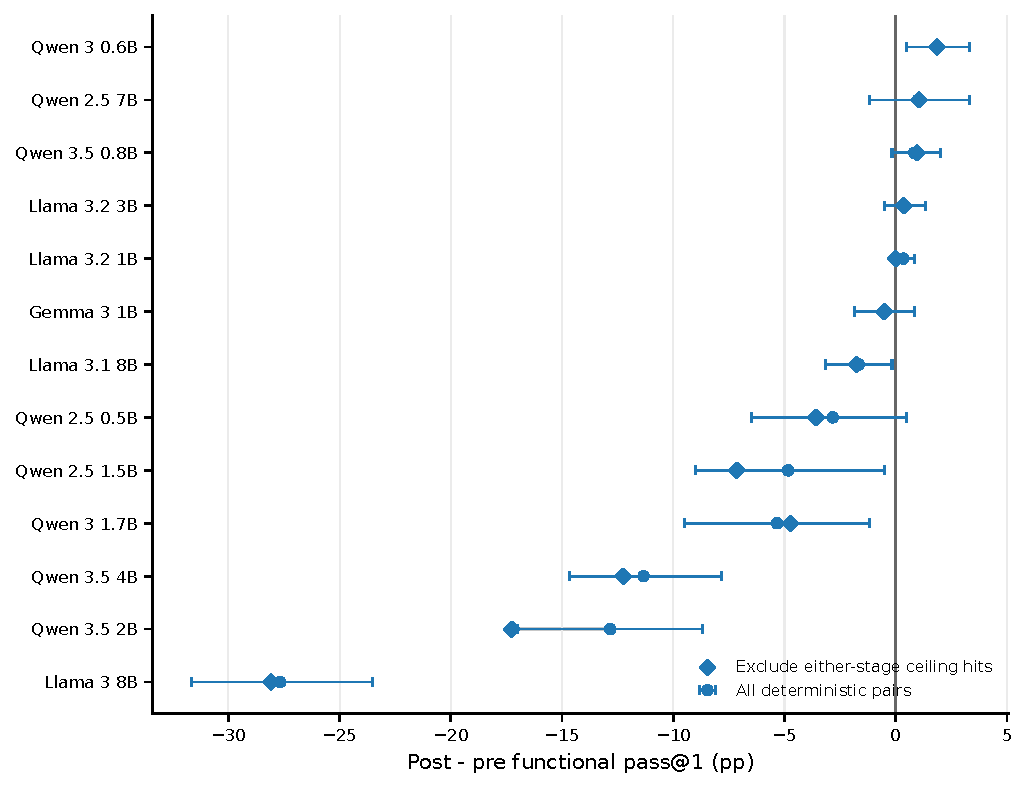
\includegraphics[width=0.52\linewidth]{fig3_mbpp_heterogeneity.pdf}
% \caption{Per-checkpoint change in deterministic MBPP pass@1 after SFT (pp).
% Circles use all 600 deterministic pairs per checkpoint with paired-bootstrap
% 95\% intervals; diamonds exclude pairs that reach the generation-ceiling
% proxy at either stage. Every checkpoint whose pre-SFT pass@1 exceeds 15\%
% declines; the checkpoints that do not decline all start below 5\%.}
% \label{fig:mbpp}
% \end{figure}
\vspace{-3mm}
\section{Discussion}
\label{sec:discussion}
\vspace{-2mm}

\noindent\textbf{Strict gains can overstate what post-training changes.}
We find that strict success combines evaluator compliance with task correctness,
which can change at different rates. In our audit, SFT increased compliance by
34.78\pp{} but strict success by only 12.12\pp{}, leaving a 22.66\pp{} increase
in valid-but-wrong responses. We therefore argue that higher benchmark scores
can reflect substantial learning of the evaluator-facing contract without a
comparable gain in task success. This does not make compliance learning
undesirable; rather, we should report what drives the score change.
\\
\noindent\textbf{Correctness depends on the instrument.}
We find that strict evaluation provides the cleanest primary outcome, while
relaxed extraction reveals additional transition structure but depends on the
extractor. Where a behavioral oracle exists, we find that it provides a
stronger capability check: on MBPP, compliance increased while functional
correctness declined. We therefore view these measures as complementary rather
than interchangeable estimates of correctness.
\\
\noindent\textbf{Implications for evaluation.}
We recommend that benchmarks with output contracts report pre- and post-training
compliance \(F\), strict success \(S\), and valid-but-wrong rate \(F-S\). We
also recommend retaining item-level transitions and versioning contract
checkers and relaxed extractors separately. Where a behavioral oracle exists,
we suggest using it to anchor capability claims. These additions complement,
rather than replace, strict accuracy.
\\
\noindent\textbf{Limitations.}
We study heterogeneous, single-run SFT interventions rather than a controlled
experimental design. Complete training-dose metadata are available for only
five of 55 model--task blocks, so our results do not isolate the effect of a
specific SFT recipe or imply a universal format--capability trade-off. Since
the output convention appears in the SFT targets, the observed compliance
gains are also tied to the exposed contract. Controlled dose sweeps, training
seeds, and supervision ablations would further separate interface learning
from capability changes, forgetting, and overfitting.
Also, parser-derived correctness for invalid non-MBPP outputs is not human-validated.
MBPP uses the original benchmark assertions rather than augmented suites, and
its generation-ceiling analysis uses a token-count proxy. Finally, our study
covers four English benchmarks and models up to 8B parameters, so results may
vary across languages, model scales, contracts, and post-training methods.

\vspace{-3mm}
\section{Conclusion}
\label{sec:conclusion}
\vspace{-2mm}
Strict accuracy remains an important metric, but it does not reveal why a score
changes. CCD makes this distinction explicit by separating compliance, strict
success, and the valid-but-wrong state using matched pre- and post-training
outputs. Across 49{,}140 matched responses, compliance increased nearly three
times as much as strict success, with a 22.66\pp{} increase in valid-but-wrong
responses. On MBPP, an independent execution-based measure shows that higher
compliance can coexist with lower functional correctness. Together, these
results support a simple evaluation principle: \emph{report whether models
learned to satisfy the evaluator, became more correct, or both.}


\bibliographystyle{plainnat}
\bibliography{references}
\clearpage
\newpage
\appendix

\section{Related Work}
\label{sec:related_work}

\noindent\textbf{Format-aware and multidimensional evaluation.}
Recent work has shown that a single benchmark score can hide important
differences in model behavior. HELM evaluates models across multiple scenarios
and desiderata \citep{liang2023holistic}, while IFEval isolates objectively
verifiable instruction following \citep{zhou2023ifeval}. FoFo further shows
that format following can vary independently of content quality
\citep{xia-etal-2024-fofo}. Measured performance is also sensitive to how tasks
and outputs are represented: meaning-preserving prompt changes can produce
substantial score differences \citep{sclar2024quantifying}, and equivalent
output formats can affect fine-tuned models
\citep{ravikumar-etal-2026-lost}. Most closely related, prior work
distinguishes performance with and without format adherence and studies the
effect of requested output formats \citep{long-etal-2025-llms}. These works
establish that evaluator-facing format is an important component of
measurement. We focus on a narrower question: \emph{when the evaluator and
output contract are fixed, what accounts for a score change after
post-training?}

\noindent\textbf{Structured generation and post-training.}
A substantial body of work improves or enforces structured output through
constrained decoding, prompting, or additional training. Grammar-based
decoding can guarantee formal validity \citep{geng-etal-2023-grammar}, while
CRANE combines structural constraints with intermediate reasoning
\citep{pmlr-v267-banerjee25a}. Other approaches fine-tune models for particular
output formats \citep{bunn-etal-2025-fine}, separate task solving from format
control during decoding \citep{deng-etal-2026-decoupling}, or optimize prompts
for structured output reliability \citep{galeone2026correct}. Instruction
tuning itself can improve instruction following and transfer
\citep{wei2022finetuned,sanh2022multitask,pmlr-v202-longpre23a}, with LIMA
showing that relatively small amounts of supervision can substantially shape
response conventions \citep{zhou2023lima}. Studies of SFT also report that its
effects vary with training data, model, and training stage, and that gains on
some objectives can coincide with losses on others
\citep{fu-etal-2024-disperse,harada-etal-2025-massive}. This literature
motivates separating observable dimensions of post-training change, but does
not provide an item-paired decomposition of compliance and strict correctness
under a fixed evaluator.

\noindent\textbf{Correctness beyond parsing.}
For some tasks, correctness can be assessed independently of whether the
response follows the expected textual format. In code generation, MBPP uses
test execution to evaluate generated programs \citep{austin2021program}, while
EvalPlus shows that execution-based conclusions depend on the coverage and
strength of the test suite \citep{liu2023evalplus}. Thus, parser-based validity
and functional correctness are distinct measurement instruments. Our work
retains this distinction: CCD uses the original evaluator to measure
compliance and strict success, while execution-based correctness is treated as
an independent secondary measure where available. In contrast to approaches
that modify generation, relax the evaluator, or compare alternative formats,
CCD asks how the same evaluator outcomes change across matched responses
before and after SFT. This provides a direct account of whether post-training
primarily changes compliance, strict success, or the population of responses
that are compliant but still incorrect.

\begin{table}[t]
\centering
\caption{\textbf{Positioning CCD relative to closely related evaluation and
structured-output studies.} A check mark indicates that the feature is an
explicit part of the study; a dash indicates that it is not a primary
analysis. ``Transitions'' denotes matched, item-level changes between
conditions, and ``behavioral oracle'' denotes execution-based correctness.}
\label{tab:related_comparison}

\scriptsize
\setlength{\tabcolsep}{3pt}
\renewcommand{\arraystretch}{1.12}

\begingroup
\newcommand{\yes}{\(\checkmark\)}
\newcommand{\no}{\textemdash}

\begin{tabularx}{\linewidth}{
    @{}
    p{1.75cm}
    Y
    >{\centering\arraybackslash}m{1.15cm}
    >{\centering\arraybackslash}m{1.25cm}
    >{\centering\arraybackslash}m{1.45cm}
    >{\centering\arraybackslash}m{1.25cm}
    @{}
}
\toprule
Work &
Primary comparison &
\makecell[tc]{Contract\\fixed} &
\makecell[tc]{Item-level\\transitions} &
\makecell[tc]{Wrong-valid\\outcome} &
\makecell[tc]{Behavioral\\oracle} \\
\midrule

FoFo \citep{xia-etal-2024-fofo}
& Models across domain-specific formats
& \no & \no & \no & \no \\

Long et al.~\citep{long-etal-2025-llms}
& Requested formats and mitigation methods
& \no & \no & \no & \no \\

Bunn et al.~\citep{bunn-etal-2025-fine}
& Standard versus format-specific fine-tuning
& \yes & \no & \no & \no \\

Deng et al.~\citep{deng-etal-2026-decoupling}
& Standard versus decoupled decoding
& \yes & \no & \no & \no \\

Galeone et al.~\citep{galeone2026correct}
& Prompting and constrained-generation strategies
& \yes & \no & \no & \no \\

Ray~\citep{ray2026constrainttax}
& Prompt-only versus hard-schema control
& \yes & \no & \yes & \yes \\

\midrule

\textbf{CCD (ours)}
& \textbf{Matched pre- versus post-SFT responses}
& \yes & \yes & \yes & \yes \\

\bottomrule
\end{tabularx}

\endgroup
\end{table}

\section{Reproducibility statement}
\label{app:reproducibility_statement}
The accompanying reproducibility materials include retained pre- and post-SFT
generations, 49{,}140 paired item-level records, cell-level results, execution
labels for 11{,}700 paired MBPP programs, and documented evaluation settings.
These materials support reproduction of the reported tables, figures,
confidence intervals, transition matrices, and sensitivity analyses without
repeating model training or generation. They also support verification of the
strict-score identity (Eq.~\ref{eq:identity}) and the paired flow decomposition
(Eq.~\ref{eq:gap_flow}). Exact reproduction of every historical SFT run remains
limited by incomplete training metadata for 50 of the 55 model--task evaluation
blocks (Appendix~\ref{app:audit}).

The materials additionally include a stratified 300-item parser-audit sample
and a two-annotator protocol. The sample contains 75 pre-SFT items per benchmark,
balanced across extractor states where coverage permits. Human annotation and
adjudication have not been completed; no agreement statistics or human-validated
correctness claims are based on this sample.

\noindent\textbf{Minimal replication.}
The headline result requires only that records be paired by stable item ID
within each model $\times$ dataset $\times$ configuration cell, that $F$ and
$S$ be computed at both stages, and that cell-level deltas be averaged under
the stated weighting. The four-state analysis additionally requires the
versioned relaxed-extractor output $\Crel$; the MBPP analysis requires the
execution status of each candidate. A replication should retain, for every
item, the model label and loader ID, dataset and item ID, configuration,
stage, raw prompt and completion, extracted answer, gold answer, format flag,
correctness flag, strict flag, generated-token count, and, where applicable,
execution status and error class; for self-consistency, the sampled
candidates, their parsed answers and format flags, the selected winner, and
the tie-breaking rule. Run-level records should include seed, maximum
sequence length, maximum new tokens, training-set size, maximum steps,
effective batch, learning rate, adapter configuration, and package versions.


\section{More Details on Evaluation Design}
\label{app:Evaluation-Design}
Here, we define how CCD decomposes post-training change. We now specify the evaluation design that makes this decomposition comparable across stages. Before- and after-SFT records must refer to the same item under the same prompt construction, inference procedure, and evaluator, while historical differences in evaluator versions and SFT recipes must remain visible. This design supports an audit of recorded outcomes across models, tasks, and inference settings without obscuring the scope of each claim.

\subsection{Models, Benchmarks, and Inference Configurations}

\noindent\textbf{Models.}
We evaluate 14 instruction-tuned models spanning approximately 270M to 8B parameters. The model set comprises Gemma 3 at 270M and 1B parameters; Llama 3 at 8B, Llama 3.1 at 8B, and Llama 3.2 at 1B and 3B; Qwen 2.5 at 0.5B, 1.5B, and 7B; Qwen 3 at 0.6B and 1.7B; and Qwen 3.5 at 0.8B, 2B, and 4B \citep{gemmateam2025gemma3,dubey2024llama3,qwenteam2024qwen25,qwenteam2026qwen35,yang2025qwen3}. Every run uses four-bit weight loading with low-rank adapters \citep{dettmers2023qlora}. Table~\ref{tab:checkpoints} lists the canonical loader identifier associated with each analytical model label; dataset-specific names retained in historical files are treated as provenance fields, not as additional models.

\noindent\textbf{Benchmarks and output contracts.}
We use four benchmarks with different answer types and correctness mechanisms: GSM8K for numerical reasoning \citep{cobbe2021training}, LogiQA for multiple-choice logical reasoning \citep{liu2020logiqa}, MBPP for Python program synthesis \citep{austin2021program}, and StrategyQA for implicit Boolean reasoning \citep{geva-etal-2021-aristotle}. This variation is important for the paper's central question. A compliance gain tied only to one answer representation would be qualitatively different from a pattern that recurs across numbers, option labels, Boolean answers, and programs.

\noindent\textbf{Inference configurations.}
Each available model--task block is evaluated before and after SFT under nine prespecified configurations: direct zero-shot prompting (Zero), zero-shot chain-of-thought prompting (CoT; \citealp{kojima2022large}), few-shot prompting with \(k\in\{0,1,3,5\}\) demonstrations (\(\mathrm{FS}_k\); \citealp{brown2020language}), and self-consistency with \(k\in\{1,3,5\}\) sampled reasoning paths (\(\mathrm{SC}_k\); \citealp{wang2023selfconsistency}). \(\mathrm{FS}_0\) retains the few-shot scaffold with an empty demonstration block and is therefore distinct from Zero. Zero, CoT, and few-shot configurations use greedy decoding; self-consistency samples candidates and votes over their extracted answers. Pre-SFT and post-SFT refer to evaluation immediately before and after fine-tuning.

\begin{table*}[t]
    \caption{\textbf{Output contracts and evaluation criteria.}
    Strict success $S$ requires both compliance with the specified output
    contract and acceptance under the corresponding strict criterion
    (Equation~\eqref{eq:identity}). Fallback extraction is used only for the secondary
    parser-derived analysis described in Section~\ref{sec:instruments}. MBPP functional claims
    use standardized execution $C^{\mathrm{func}}$, rather than the archived
    correctness flag.}
    \label{tab:output_contracts}

    \centering
    \small
    \setlength{\tabcolsep}{6pt}
    \renewcommand{\arraystretch}{1.18}

    \begin{tabularx}{\textwidth}{
        @{}
        >{\raggedright\arraybackslash}p{0.12\textwidth}
        >{\raggedright\arraybackslash}p{0.09\textwidth}
        Y
        Y
        @{}
    }
        \toprule
        \textbf{Benchmark} &
        \textbf{Output} &
        \textbf{Required contract} &
        \textbf{Strict criterion} \\
        \midrule

        GSM8K &
        Number &
        \texttt{Final Answer: \textless number\textgreater} &
        Normalized numeric match \\
        \addlinespace[2pt]

        StrategyQA &
        Yes/No &
        \texttt{Final Answer: Yes\textbar No} &
        Label match \\
        \addlinespace[2pt]

        LogiQA &
        Option &
        \texttt{Final Answer: A\textbar B\textbar C\textbar D} &
        Option match \\
        \addlinespace[2pt]

        MBPP &
        Program &
        Final-answer boundary followed by Python code &
        Archived evaluator verdict; standardized execution reported separately \\
        
        \bottomrule
    \end{tabularx}
\end{table*}



\subsection{Paired Design and Item Selection}

The archive yields 49,140 matched pre-/post-SFT response pairs distributed across 495 evaluation cells and 55 model--task blocks. One otherwise expected block, Qwen 2.5 7B on LogiQA, has no retained item-level records. Of the 495 observed cells, 477 contain 100 matched pairs and 18 contain 80; the smaller cells correspond to Qwen 2.5 7B on GSM8K and StrategyQA.

Pairs are formed using stable task identifiers or explicit item indices whenever available. When neither is retained, we require agreement in item order, question text, and reference answer before accepting the alignment. Official training and evaluation partitions remain separate throughout. GSM8K and StrategyQA use the first \(n\) retained evaluation items, whereas LogiQA and MBPP are shuffled with seed 42 before item selection.

The historical runs generated up to 100 pre-SFT and 200 post-SFT records per configuration. We do not compare these unequal sets directly. Instead, each analysis cell uses only the identity-matched intersection of items present at both stages, preventing additional post-SFT records from changing the comparison set. This restriction also limits the estimand: request failures were not logged consistently enough to justify a missing-at-random assumption, so all reported changes are conditional on the retained pairs rather than estimates for unobserved generations.

\subsection{Contract Checking and Parser-Derived Extraction}

The strict evaluator operationalizes the two primary CCD variables. It sets compliance \(F\) from the required answer boundary and representation, and it assigns strict success \(S\) only when a compliant response also satisfies the task-specific criterion in Table~\ref{tab:output_contracts}. A contract-invalid response never receives strict credit, even if a secondary extractor can recover a plausible answer.

The parser-derived instrument \(C^{\mathrm{rel}}\) applies a deterministic fallback when the required answer region is absent or unusable. For GSM8K, it takes the last normalized numeric match in the completion; for StrategyQA, it searches for a standalone Yes or No label; for LogiQA, it searches for an explicit option from A to D; and for MBPP, it uses the final fenced Python block or, if no such block exists, the completion itself. Appendix~\ref{app:instrument_full} specifies the exact normalization and matching rules. These fallback outputs support the secondary four-state analysis, but they do not alter \(F\) or the strict-success outcome.

Self-consistency requires additional version tracking. Each candidate is parsed separately before voting. Earlier harnesses mark the aggregate as compliant when any sample is compliant, even if it does not support the winner; later harnesses require a compliant sample among the winner's supporters. Program voting likewise uses either normalized source text or abstract-syntax-tree normalization. We preserve each record's original rule and use greedy-only analyses to test sensitivity to these differences.

All extractors are deterministic and versioned, and all 49,140 pairs satisfy the strict-success identity \(S=FC^{\mathrm{rel}}\) at both stages. Parser-derived labels for contract-invalid natural-language responses have not been validated against human judgments. The release includes a stratified 300-item sample---75 pre-SFT items per benchmark, balanced across extractor states where possible---and a two-annotator protocol, but annotation and adjudication are incomplete. We therefore make no human-validated correctness or agreement claim; the primary CCD analysis does not depend on this sample.

\subsection{Scope of the Post-Training Intervention}

The paired design is controlled at evaluation time, but the underlying SFT interventions do not follow one standardized recipe. Adapter scaling, dropout, training budget, and data construction vary, and some model--task blocks share an adapter. The 55 evaluation blocks are therefore neither 55 independent training runs nor repeated estimates of a common treatment.

All fields required to reconstruct training dose---training-set size, maximum steps, train batch size, and gradient accumulation are jointly available for only five of the 55 model--task blocks. Missing settings are left empty rather than imputed, and recovered configurations are reported in Table~\ref{tab:dose_recovered_full}. The study therefore estimates paired changes across the observed interventions; it does not identify a dose--response relation or the causal effect of a standardized SFT procedure.

Training targets also contain the same final-answer convention required by the evaluator. Compliance changes therefore describe behavior under an explicitly supervised, evaluation-matched contract; they do not measure transfer to unseen output schemas. CCD asks whether increased adherence to this exposed interface is accompanied by strict success, but its conclusions should not be extended beyond the evaluated contracts.

\subsection{Standardized Functional Evaluation on MBPP}
\label{sec:mbpp_design}

Archived MBPP correctness is not a uniform measure of program behavior: earlier harnesses compare normalized source strings, whereas later versions execute extracted programs. To obtain a common functional criterion, we re-execute every selected candidate for which the task-to-test mapping can be verified. Thirteen checkpoints meet this requirement, producing 117 cells and 11,700 matched program pairs. Gemma 3 270M is excluded because its retained records cannot be linked uniquely to the standardized mapping.

Each extracted program is evaluated against the original MBPP assertions, rather than an EvalPlus-augmented test suite \citep{liu2023evalplus}. Every candidate remains in the denominator; empty or malformed code, execution errors, timeouts, and failed assertions are all counted as failures. This standardized outcome is \(C^{\mathrm{func}}\) from Equation~\eqref{eq:functional}, and it is evaluated independently of compliance.

The distinction from the archived flag is substantive. The full 14-checkpoint pre-SFT MBPP archive contains 12,600 records; 8,100 have no execution status and carry an incorrect archived label. We retain those labels when auditing strict evaluator outcomes, because CCD's primary question concerns what the evaluator recorded, but use standardized re-execution exclusively for functional claims. Missing historical execution is therefore not treated as evidence that a program fails its tests.

For deterministic configurations, functional performance is reported as pass@1. Summaries that also include self-consistency describe the selected program after voting among sampled candidates and are therefore reported as \textbf{selected-output functional accuracy}, not conventional pass@1. We additionally test whether any functional change is explained by truncation. A candidate is marked as reaching the generation ceiling when its generated-token count equals the model's repeated hard upper bound of 256 or 384 tokens; the functional comparison is then repeated after removing every pair with a ceiling hit at either stage.

\subsection{Analysis Implementation and Provenance}

Cell-level estimands, equal-cell aggregation, hierarchical bootstrap intervals, paired tests, and robustness analyses follow Section~\ref{sec:aggregation}. Their implementation operates entirely on retained paired records and requires no additional model generations. Before analysis, we verify Equation~\eqref{eq:identity} for every response at both stages and reproduce each observation-weighted compliance--success gap from the corresponding transition counts.

The provenance audit separates item-level evidence from historical aggregate exports. The archived workbook contains 1,148 rows for 1,008 intended model--task--stage--configuration keys because 140 keys occur in more than one export. The audit layer records explicit source precedence, but no paired result is calculated from these competing aggregate rows; all results are recomputed from the item-level files, preventing duplicate exports from entering the analysis.

Finally, each of the 55 observed model--task blocks has a manifest recording its source files, pairing key, item count, seed, decoding settings, and SHA-256 file identities. The accompanying materials include the retained generations, 49,140 paired records, execution outcomes for 11,700 MBPP pairs, cell summaries, and analysis scripts. These materials reproduce the evaluation audit, but they do not remove the stated limitation that most historical training runs cannot be reconstructed fully.

\subsection{Models, run settings, and audit trail}
\label{app:checkpoints}
Each analytical model label denotes one model used consistently across
benchmarks (Table~\ref{tab:checkpoints}). All runs use four-bit weight loading,
including checkpoints whose repository names do not specify a quantization
format.

\begin{table}[h]
\centering
\small
\setlength{\tabcolsep}{5pt}
\begin{tabular}{llr}
\toprule
\textbf{Analytical label} & \textbf{Canonical checkpoint / loader ID} & \textbf{Params (B)}\\
\midrule
Gemma 3 270M  & \texttt{unsloth/gemma-3-270m-it-bnb-4bit} & 0.27\\
Gemma 3 1B    & \texttt{unsloth/gemma-3-1b-it-bnb-4bit} & 1.0\\
Llama 3 8B    & \texttt{unsloth/llama-3-8b-Instruct-bnb-4bit} & 8.0\\
Llama 3.1 8B  & \texttt{unsloth/Meta-Llama-3.1-8B-Instruct-bnb-4bit} & 8.0\\
Llama 3.2 1B  & \texttt{unsloth/Llama-3.2-1B-Instruct-bnb-4bit} & 1.0\\
Llama 3.2 3B  & \texttt{unsloth/Llama-3.2-3B-Instruct-bnb-4bit} & 3.0\\
Qwen 2.5 0.5B & \texttt{unsloth/Qwen2.5-0.5B-Instruct-bnb-4bit} & 0.5\\
Qwen 2.5 1.5B & \texttt{unsloth/Qwen2.5-1.5B-Instruct-bnb-4bit} & 1.5\\
Qwen 2.5 7B   & \texttt{unsloth/Qwen2.5-7B-Instruct-bnb-4bit} & 7.0\\
Qwen 3 0.6B   & \texttt{unsloth/Qwen3-0.6B-unsloth-bnb-4bit} & 0.6\\
Qwen 3 1.7B   & \texttt{unsloth/Qwen3-1.7B-unsloth-bnb-4bit} & 1.7\\
Qwen 3.5 0.8B & \texttt{unsloth/Qwen3.5-0.8B} & 0.8\\
Qwen 3.5 2B   & \texttt{unsloth/Qwen3.5-2B} & 2.0\\
Qwen 3.5 4B   & \texttt{unsloth/Qwen3.5-4B} & 4.0\\
\bottomrule
\end{tabular}
\caption{\textbf{One canonical checkpoint per analytical model label.} Dataset-specific
strings retained in historical output tables are provenance fields, not
distinct checkpoints.}
\label{tab:checkpoints}
\end{table}

\subsubsection{Audit trail and recovered run settings}
\label{app:audit}
The design manifest links each paired model $\times$ dataset evaluation to its
source files, row counts, pairing key, seed, and decoding settings; a separate
audit layer retains SHA-256 file identities and reconciles historical
aggregate exports. For historical auditing only, the aggregate workbook
contains 1{,}148 rows for 1{,}008 intended model $\times$ dataset $\times$
stage $\times$ configuration keys because 140 keys have more than one retained
export; the audit layer records explicit source precedence, and all paired
results in the paper are computed from item-level files rather than from
competing aggregate exports.

The completed SFT recipes are heterogeneous. The manifest records each run's
settings where they were recovered and leaves fields explicitly empty rather
than imputed otherwise. All four fields needed to reconstruct training dose
(training-set size, maximum steps, train batch, gradient accumulation) are
available for five of the 55 model--task blocks, including one MBPP block
(Table~\ref{tab:dose_recovered_full}); these rows also use LoRA rank and alpha
16/16, learning rate $10^{-4}$, train batch 1, and gradient accumulation 16.
Effective epochs are $E_{\mathrm{eff}}=\text{steps}\times
B_{\mathrm{train}}A_{\mathrm{grad}}/N_{\mathrm{train}}$.

\begin{table}[h]
\centering
\small
\setlength{\tabcolsep}{4pt}
\begin{tabular}{llrrrrrrr}
\toprule
\textbf{Model} & \textbf{Dataset} & \textbf{Train $N$} & \textbf{Steps} & \textbf{Max seq} & \textbf{Max new} & \textbf{Eff.\ epochs} & $\boldsymbol{\Delta\Crel}$ & $\boldsymbol{\Drel}$\\
\midrule
Llama 3 8B    & StrategyQA & 400  & 220 & 1024 & 40  & 8.8  & $+1.00$  & \ccdheat{20}$-0.44$\\
Qwen 3.5 0.8B & LogiQA     & 1500 & 300 & 2048 & 96  & 3.2  & $+19.00$ & \ccdheat{65}$+33.44$\\
Qwen 3.5 0.8B & MBPP       & 300  & 300 & 2048 & 384 & 16.0 & $+0.67$  & \ccdheat{37}$+11.89$\\
Qwen 3.5 4B   & GSM8K      & 1500 & 300 & 1024 & 160 & 3.2  & $+16.00$ & \ccdheat{42}$+16.22$\\
Qwen 3.5 4B   & StrategyQA & 500  & 300 & 1024 & 40  & 9.6  & $+11.22$ & \ccdheat{8}$-9.78$\\
\bottomrule
\end{tabular}
\caption{\textbf{The five model--dataset recipes with complete dose metadata.} Deltas
average the nine inference configurations of each recipe. Five rows, one of
them MBPP, do not support a study-wide dose--response analysis: the descriptive
Spearman correlation between $\Drel$ and effective epochs is $\rho=-.67$
($p=.22$) and between $\Drel$ and maximum steps $\rho=.35$ ($p=.56$), with
task and model confounded with dose. We report these values only to show why
no dose claim is made.
Green shading (\ccdlegend{}) highlights larger values of $\Drel$ only.}
\label{tab:dose_recovered_full}
\end{table}

\section{Instrument specification}
\label{app:instrument_full}
This appendix states the scoring rules at the level needed to reproduce the
$(C,F)$ state assignments. The goal is not to prescribe a universal parser but
to make explicit which instrument produced the reported numbers.

\noindent\textbf{GSM8K.}
The contract requires an explicit \texttt{Final Answer:} boundary followed by a
number. After comma removal the numeric pattern is
\verb|-?\d+(?:\.\d+)?|. With the boundary present, the parser takes the last
numeric match inside the boundary region. Without it, the relaxed extractor
takes the last numeric match in the full completion and sets $F=0$.
The numeric parser normalizes answer strings by removing commas and a
trailing period; they do not generally canonicalize decimal representations
such as \texttt{2} and \texttt{2.0}. The analysis retains the recorded labels.

\noindent\textbf{StrategyQA.}
The contract requires \texttt{Final Answer: Yes} or \texttt{Final Answer: No}.
The strict parser searches the final-answer region for a standalone
\texttt{yes} or \texttt{no}. Without the boundary, the relaxed extractor
searches the full completion and returns a recovered label with $F=0$.
The Boolean parser checks \texttt{yes} before \texttt{no} and defaults to
\texttt{No} with $F=0$ when neither is found. Because this can credit an
output without an explicit answer, these labels are used only in the
parser-derived analysis.

\noindent\textbf{LogiQA.}
The contract requires one option letter A--D after the final-answer marker.
The strict parser searches the answer region for \verb|\b([ABCD])\b|; the
relaxed path searches the full completion for explicit option letters and uses
the recovered option with $F=0$. Correctness compares normalized letters.

\noindent\textbf{MBPP.}
The contract requires the final-answer boundary before the returned Python
candidate. Without the marker, the extractor retains the final fenced Python
block when present, otherwise the completion, and sets $F=0$. Code-fence
markup is stripped and the candidate is trimmed to a probable Python start.
The archived correctness label comes from the retained evaluator: earlier
implementations use normalized source-string equality, while execution-enabled
versions use test outcomes. Execution status is absent for 8{,}100 of the
12{,}600 pre-SFT records, which carry an incorrect archived label;
the standardized re-execution of Section~\ref{sec:mbpp_design} runs every
extracted candidate of the 13 mapped checkpoints against the original
assertions and credits 1{,}430 pre-SFT and 1{,}053 post-SFT candidates that
the archived flag does not. Non-executable outputs remain failures under
both. The archived flag and the re-execution metric are kept separate
throughout.

\noindent\textbf{Self-consistency.}
Each sampled candidate is parsed separately. Earlier evaluators vote over
normalized extracted answers (normalized source text for code); if the
largest vote counts tie, their helper returns the first sampled prediction.
Their format flag is the logical OR over all sampled format flags, including
samples that do not support that prediction. Later evaluators choose a most
frequent prediction with first-occurrence tie breaking and require a compliant
sample among its supporters. Execution-enabled programming evaluators vote
using abstract-syntax-tree normalization where parsing succeeds and normalized
source otherwise; they prefer a compliant program within the winning group.
The archived analysis preserves these distinctions. Thus a self-consistency
record describes a harness-level decision and need not represent one raw
completion under every version. Greedy-only summaries provide a sensitivity
that avoids sample-aggregation differences. Programming summaries that include
voted outputs are reported as selected-output functional accuracy rather than
conventional pass@1.

\section{Additional primary and parser-derived summaries}
\label{app:secondary}

\subsection{Cell-level significance counts}
\label{app:significance}

\begin{table}[H]
\centering
\small
\setlength{\tabcolsep}{6pt}

\begin{tabular}{lrrrr}
\toprule
\textbf{Outcome}
& $\boldsymbol{\Delta}$ \textbf{(pp)}
& \textbf{FDR-significant $+$}
& \textbf{FDR-significant $-$}
& \textbf{Total} \\
\midrule
Compliance $F$
& \ccdheat{65}$+34.78$ & 274 & 16 & 290 \\

Strict success $S$
& \ccdheat{24}$+12.12$ & 176 & 7 & 183 \\

Parser-derived $\Crel$
& \ccdheat{8}$+3.57$ & 54 & 13 & 67 \\
\bottomrule
\end{tabular}

\caption{\textbf{Equal-cell changes and the number of the 495 cells whose
paired change is significant under an exact McNemar test with
Benjamini--Hochberg control at $q<.05$, split by sign.}
Green shading (\ccdlegend{}) highlights larger changes in the
$\Delta$ column only.}
\label{tab:significance}
\end{table}


\subsection{Transition taxonomy}
\label{app:transition_pooled}
Table~\ref{tab:transition_main} gives the exhaustive pooled taxonomy behind
Figure~\ref{fig:transition}, and Table~\ref{tab:transition_dataset_counts}
gives raw counts by benchmark. LogiQA has the largest joint-gain count,
StrategyQA the most trade-offs, and MBPP's parser-level view is dominated by
unchanged items and pure compliance gains, which motivates the separate
execution analysis. GSM8K is the one benchmark whose pure correctness-loss
share (7.76\%) exceeds its pure correctness-gain share (7.05\%), even though
its strict success still rises because compliance gains are far more common.

\begin{table}[ht]
\centering
\small
\setlength{\tabcolsep}{6pt}
\begin{tabular}{llrr}
\toprule
\textbf{Category} & \textbf{Transitions} & \textbf{Count} & \textbf{Share}\\
\midrule
Pure compliance gain      & $\Eone\!\to\!\Etwo$, $\Ethree\!\to\!\Efour$ & 12,228 & \ccdheat{36}24.88\%\\
Pure correctness gain     & $\Eone\!\to\!\Ethree$, $\Etwo\!\to\!\Efour$ & 3,128  & \ccdheat{15}6.37\%\\
Joint gain                & $\Eone\!\to\!\Efour$                          & 3,494  & \ccdheat{16}7.11\%\\
Pure compliance loss      & $\Etwo\!\to\!\Eone$, $\Efour\!\to\!\Ethree$ & 446    & \ccdheat{9}0.91\%\\
Pure correctness loss     & $\Ethree\!\to\!\Eone$, $\Efour\!\to\!\Etwo$ & 2,894  & \ccdheat{14}5.89\%\\
Joint loss                & $\Efour\!\to\!\Eone$                          & 111    & \ccdheat{8}0.23\%\\
Trade-off                 & $\Etwo\!\leftrightarrow\!\Ethree$              & 1,970  & \ccdheat{12}4.01\%\\
Unchanged                 & diagonal                                      & 24,869 & \ccdheat{65}50.61\%\\
\bottomrule
\end{tabular}
\caption{\textbf{Exhaustive pooled taxonomy over 49{,}140 matched outputs under the
relaxed extractor.} Categories are mutually exclusive and exhaustive.
Green shading (\ccdlegend{}) highlights larger transition shares; color indicates frequency, not improvement.}
\label{tab:transition_main}
\end{table}

\begin{table}[ht]
\centering
\footnotesize
\setlength{\tabcolsep}{3pt}
\begin{tabular}{lrrrrrrrr}
\toprule
\textbf{Benchmark} & \textbf{$F$ gain} & \textbf{$C$ gain} & \textbf{Joint gain} & \textbf{Trade-off} & \textbf{$F$ loss} & \textbf{$C$ loss} & \textbf{Joint loss} & \textbf{Unchanged}\\
\midrule
GSM8K      & \ccdheat{8}2,514 & 875   & 569   & 217 & 282 & 964 & 81 & 6,918\\
LogiQA     & \ccdheat{43}3,221 & 965   & 1,579 & 575 & 42  & 820 & 12 & 4,486\\
MBPP       & \ccdheat{65}3,654 & 169   & 191   & 210 & 63  & 216 & 3  & 8,094\\
StrategyQA & \ccdheat{24}2,839 & 1,119 & 1,155 & 968 & 59  & 894 & 15 & 5,371\\
\bottomrule
\end{tabular}
\caption{\textbf{Raw transition counts by benchmark.} MBPP uses the parser-level
correctness label in this cross-task view.
Green shading (\ccdlegend{}) highlights larger counts of pure compliance gains in the $F$ gain column.}
\label{tab:transition_dataset_counts}
\end{table}

\subsection{Configuration, headroom, model, and benchmark sensitivities}
\label{app:secondary_main_tables}
\begin{table}[ht]
\centering
\small
\setlength{\tabcolsep}{6pt}
\begin{tabular}{lrrrrr}
\toprule
\textbf{Configuration} & $\boldsymbol{\Delta S}$ & $\boldsymbol{\Delta F}$ & $\boldsymbol{\Gap}$ & $\boldsymbol{\Delta\Crel}$ & $\boldsymbol{\Drel}$\\
\midrule
Zero & $+9.80$  & $+29.18$ & \ccdheat{24}$+19.39$ & $+2.36$ & $+26.82$\\
CoT  & $+14.40$ & $+35.74$ & \ccdheat{30}$+21.35$ & $+4.65$ & $+31.10$\\
FS0  & $+17.75$ & $+47.00$ & \ccdheat{58}$+29.25$ & $+5.52$ & $+41.48$\\
FS1  & $+14.40$ & $+45.61$ & \ccdheat{65}$+31.21$ & $+3.80$ & $+41.81$\\
FS3  & $+11.35$ & $+39.13$ & \ccdheat{53}$+27.78$ & $+3.16$ & $+35.97$\\
FS5  & $+6.01$  & $+20.98$ & \ccdheat{8}$+14.97$ & $+1.05$ & $+19.93$\\
SC1  & $+11.65$ & $+34.48$ & \ccdheat{36}$+22.84$ & $+3.20$ & $+31.28$\\
SC3  & $+12.14$ & $+31.49$ & \ccdheat{23}$+19.35$ & $+4.17$ & $+27.31$\\
SC5  & $+11.60$ & $+29.45$ & \ccdheat{18}$+17.85$ & $+4.18$ & $+25.27$\\
\bottomrule
\end{tabular}
\caption{\textbf{Strict and parser-derived contrasts by inference configuration (pp;
55 cells each).} FS0 is the empty-demonstration few-shot scaffold, not direct
zero-shot prompting. The compliance gain is largest for FS0 and FS1 and
smallest for FS5, whose demonstrations already induce the contract before
SFT; both gaps are positive in every configuration.
Green shading (\ccdlegend{}) highlights larger values of the primary gap $\Gap$ only.}
\label{tab:perconfig_main}
\end{table}

\begin{table}[ht]
\centering
\small
\setlength{\tabcolsep}{6pt}
\begin{tabular}{lrrrr}
\toprule
\textbf{Pre-SFT $F$ quartile} & $\boldsymbol{n}$ & \textbf{Mean pre-SFT $F$} & $\boldsymbol{\Delta F}$ & $\boldsymbol{\Drel}$\\
\midrule
Q1 (lowest)  & 124 & 0.56  & $+71.61$ & \ccdheat{65}$+66.63$\\
Q2           & 126 & 32.08 & $+57.65$ & \ccdheat{52}$+51.43$\\
Q3           & 122 & 86.20 & $+9.67$  & \ccdheat{17}$+8.10$\\
Q4 (highest) & 123 & 99.52 & $-0.85$  & \ccdheat{8}$-2.26$\\
\bottomrule
\end{tabular}
\caption{\textbf{Headroom dependence (pp).} Compliance gains, and hence the gap, are
concentrated in cells with low pre-SFT compliance and vanish where compliance
is already saturated.
Green shading (\ccdlegend{}) highlights larger values of $\Drel$ only.}
\label{tab:headroom_main}
\end{table}

\begin{table}[ht]
\centering
\small
\setlength{\tabcolsep}{6pt}
\begin{tabular}{lrrrrr}
\toprule
\textbf{Model} & $\boldsymbol{\Delta S}$ & $\boldsymbol{\Delta F}$ & $\boldsymbol{\Gap}$ & $\boldsymbol{\Delta\Crel}$ & $\boldsymbol{\Drel}$\\
\midrule
Gemma 3 270M  & $+19.42$ & $+90.83$ & \ccdheat{65}$+71.42$ & $+7.28$  & $+83.56$\\
Gemma 3 1B    & $+7.78$  & $+24.92$ & \ccdheat{20}$+17.14$ & $-1.47$  & $+26.39$\\
Llama 3 8B    & $+6.39$  & $+8.58$  & \ccdheat{8}$+2.19$  & $+4.31$  & $+4.28$\\
Llama 3.1 8B  & $+16.64$ & $+26.44$ & \ccdheat{14}$+9.81$  & $+12.61$ & $+13.83$\\
Llama 3.2 1B  & $+14.78$ & $+50.14$ & \ccdheat{35}$+35.36$ & $-1.14$  & $+51.28$\\
Llama 3.2 3B  & $+8.72$  & $+26.17$ & \ccdheat{21}$+17.44$ & $+0.72$  & $+25.44$\\
Qwen 2.5 0.5B & $+17.47$ & $+52.08$ & \ccdheat{35}$+34.61$ & $+0.81$  & $+51.28$\\
Qwen 2.5 1.5B & $+15.00$ & $+34.61$ & \ccdheat{22}$+19.61$ & $+2.81$  & $+31.81$\\
Qwen 2.5 7B   & $+18.55$ & $+67.31$ & \ccdheat{46}$+48.76$ & $+3.04$  & $+64.27$\\
Qwen 3 0.6B   & $+6.36$  & $+14.75$ & \ccdheat{13}$+8.39$  & $+0.81$  & $+13.94$\\
Qwen 3 1.7B   & $+9.17$  & $+31.47$ & \ccdheat{25}$+22.31$ & $-1.47$  & $+32.94$\\
Qwen 3.5 0.8B & $+6.75$  & $+15.92$ & \ccdheat{14}$+9.17$  & $+4.81$  & $+11.11$\\
Qwen 3.5 2B   & $+11.81$ & $+32.94$ & \ccdheat{24}$+21.14$ & $+6.69$  & $+26.25$\\
Qwen 3.5 4B   & $+12.47$ & $+18.94$ & \ccdheat{12}$+6.47$  & $+10.00$ & $+8.94$\\
\bottomrule
\end{tabular}
\caption{\textbf{Per-model equal-cell strict and parser-derived contrasts (pp),
averaged over the observed benchmark--configuration cells of each checkpoint.}
$\Gap>0$ and $\Drel>0$ for every checkpoint.
Green shading (\ccdlegend{}) highlights larger values of the primary gap $\Gap$ only.}
\label{tab:permodel}
\end{table}

\begin{table}[ht]
\centering
\small
\setlength{\tabcolsep}{5pt}
\begin{tabular}{lrrrrrr}
\toprule
\textbf{Omitted benchmark} & \textbf{Cells} & $\boldsymbol{\Delta S}$ & $\boldsymbol{\Delta F}$ & $\boldsymbol{\Gap}$ & $\boldsymbol{\Delta\Crel}$ & $\boldsymbol{\Drel}$\\
\midrule
GSM8K      & 369 & $+14.84$ & $+38.68$ & \ccdheat{49}$+23.83$ & $+4.20$ & $+34.47$\\
LogiQA     & 378 & $+10.32$ & $+31.51$ & \ccdheat{15}$+21.18$ & $+1.63$ & $+29.88$\\
MBPP       & 369 & $+15.32$ & $+35.91$ & \ccdheat{8}$+20.59$ & $+4.91$ & $+31.00$\\
StrategyQA & 369 & $+8.04$  & $+33.12$ & \ccdheat{65}$+25.08$ & $+3.57$ & $+29.56$\\
\bottomrule
\end{tabular}
\caption{\textbf{Leave-one-benchmark-out sensitivity (pp).} Strict columns follow from
the per-benchmark equal-cell means in Table~\ref{tab:headline}. Both gaps
remain positive after removing any task family.
Green shading (\ccdlegend{}) highlights larger values of the primary gap $\Gap$ only.}
\label{tab:lodo}
\end{table}

Leaving one model out at a time (Table~\ref{tab:robust_main}) gives
$\Delta S\in[11.55,12.57]$, $\Delta F\in[30.39,36.84]$,
$\Gap\in[18.84,24.27]$, $\Delta\Crel\in[2.86,3.96]$, and
$\Drel\in[27.11,33.33]$\pp{}; the smallest gaps arise when Gemma~3~270M is
omitted and the largest when Llama~3~8B is omitted. Weighting changes the
picture even less: equal-cell, observation-weighted, and equal-model summaries
give $\Drel=31.22$, $31.10$, and $31.81$\pp{}.

\subsection{Within-benchmark coupling of compliance and correctness}
\label{app:withindataset}
Figure~\ref{fig:scatter} visualizes cell-level coupling,
Table~\ref{tab:within_main} reports the benchmark-level statistics, and
Table~\ref{tab:conditional_df} stratifies correctness changes by the size of
the compliance change.
\begin{figure}[ht]
\centering
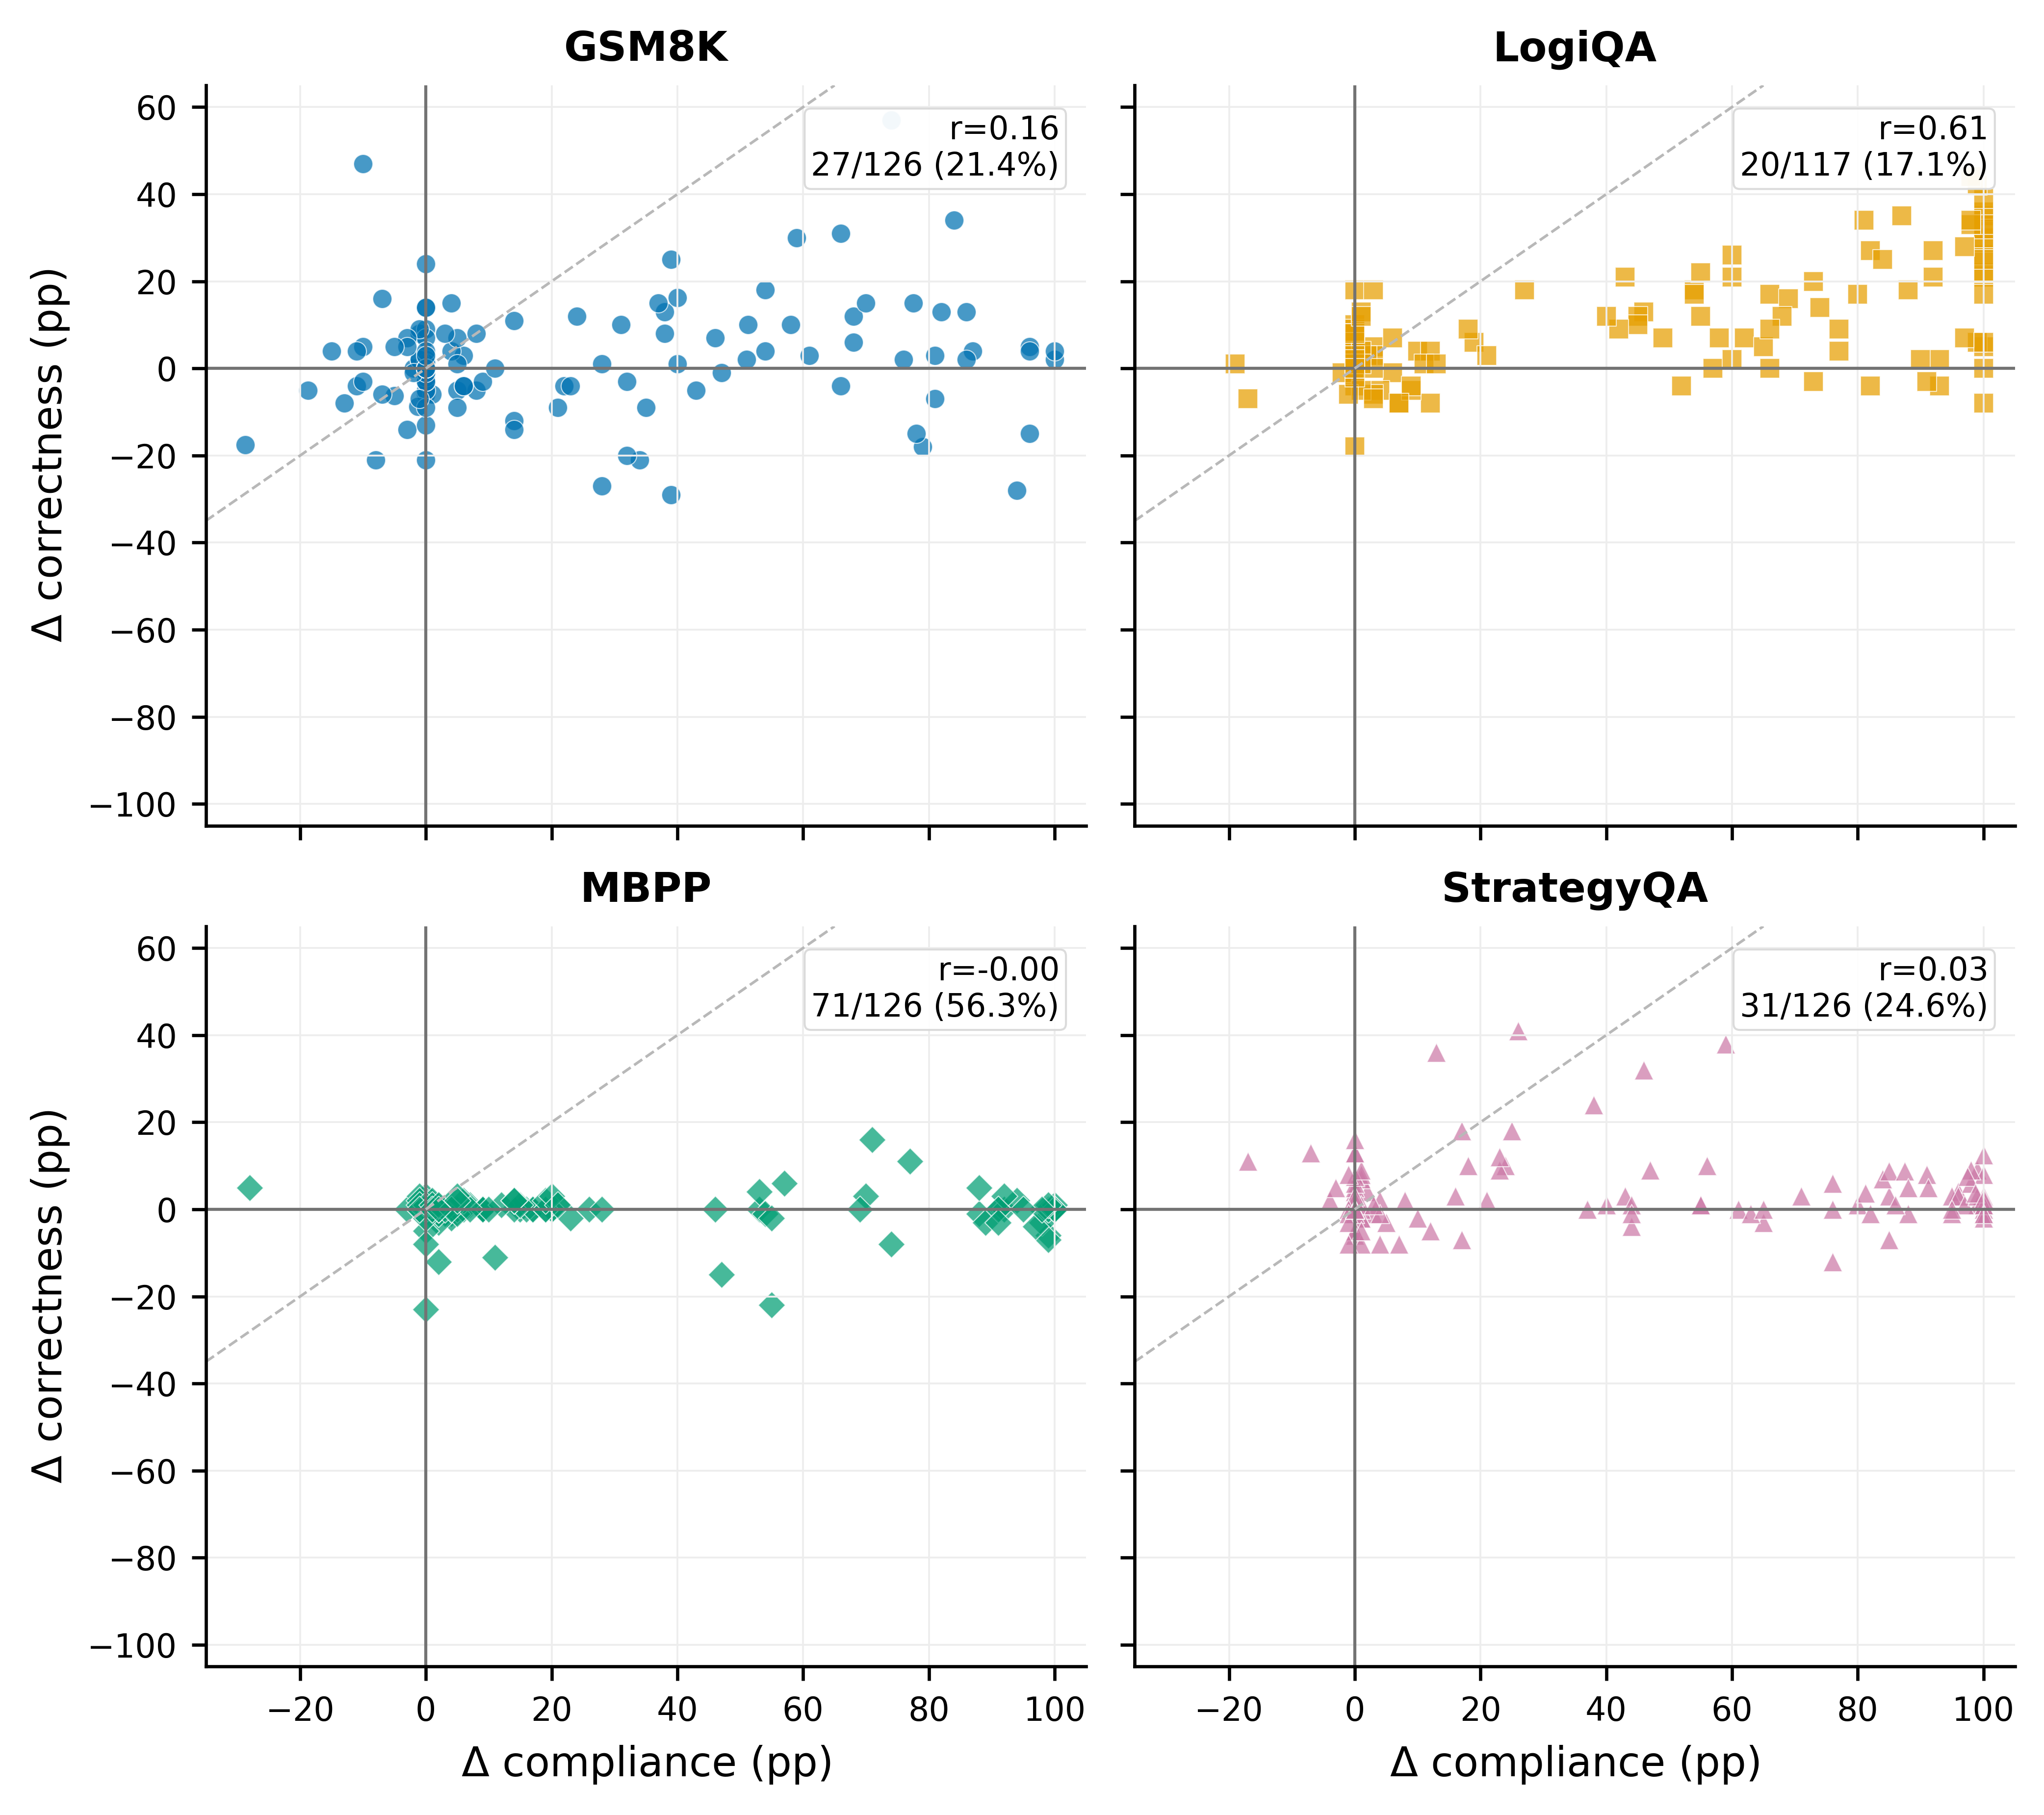
\includegraphics[width=0.9\linewidth]{Scatter4Figure.png}
\caption{\textbf{Cell-level changes in compliance ($\Delta F$) and parser-derived
correctness ($\Delta\Crel$) for the 495 cells, by benchmark.} Annotations give
the Pearson correlation and the number of cells with $\Delta F>0$ and
$\Delta\Crel\le0$; the dashed diagonal marks equal changes.}
\label{fig:scatter}
\end{figure}

\begin{table}[ht]
\centering
\small
\setlength{\tabcolsep}{5pt}
\begin{tabular}{lrrrrr}
\toprule
\textbf{Benchmark} & \textbf{Cells} & \textbf{Pearson $r$} & \textbf{Spearman $\rho$} & $\boldsymbol{\Delta F>0,\ \Delta\Crel\le0}$ & \textbf{Mean $\Drel$ (pp)}\\
\midrule
GSM8K      & 126 & $.16$ & $.18$    & \ccdheat{14}27/126 (21.4\%) & 21.68\\
LogiQA     & 117 & $.61$ & $.55$    & \ccdheat{8}20/117 (17.1\%) & 35.56\\
MBPP       & 126 & $-.00$ & $-.11$  & \ccdheat{65}71/126 (56.3\%) & 31.86\\
StrategyQA & 126 & $.03$ & $.12$    & \ccdheat{19}31/126 (24.6\%) & 36.09\\
\midrule
Pooled     & 495 & $.28$ & $.24$    & \ccdheat{27}149/495 (30.1\%) & 31.22\\
\bottomrule
\end{tabular}
\caption{\textbf{Within-benchmark coupling between $\Delta F$ and $\Delta\Crel$.} On
the 117-cell functional MBPP subset the corresponding values are $r=.23$,
$\rho=.16$, 64/117 cells (54.7\%) with $\Delta F>0$ and $\Delta\Cfunc\le0$,
and mean $\Dfunc=30.87$\pp{}. Partial correlations that control for pre-SFT
levels are $.23$, and $.17$ with benchmark fixed effects.
Green shading (\ccdlegend{}) highlights larger percentages of cells with $\Delta F>0$ and $\Delta\Crel\le0$; other columns are unshaded.}
\label{tab:within_main}
\end{table}

\begin{table}[ht]
\centering
\small
\setlength{\tabcolsep}{6pt}
\begin{tabular}{lrrr}
\toprule
$\boldsymbol{\Delta F}$ \textbf{quartile} & $\boldsymbol{n}$ & \textbf{Mean $\Delta F$} & \textbf{Mean $\Delta\Crel$}\\
\midrule
Q1 (lowest)  & 124 & $-2.34$  & \ccdheat{12}$+0.88$\\
Q2           & 124 & $+4.31$  & \ccdheat{8}$+0.40$\\
Q3           & 123 & $+44.00$ & \ccdheat{55}$+5.93$\\
Q4 (highest) & 124 & $+93.23$ & \ccdheat{65}$+7.07$\\
\bottomrule
\end{tabular}
\caption{\textbf{Parser-derived correctness change conditional on the size of the
compliance change (pp).} Even the cells with the largest compliance gains show
correctness gains an order of magnitude smaller.
Green shading (\ccdlegend{}) highlights larger mean correctness changes $\Delta\Crel$ only.}
\label{tab:conditional_df}
\end{table}

\subsection{Extractor sensitivity}
\label{app:parser_dataset}
Table~\ref{tab:parser_threeway} repeats the pooled contrast under three
correctness rules, and Table~\ref{tab:parser_dataset_sens} splits the strict
and current rules by benchmark. The largest attenuation occurs on StrategyQA,
where a Yes/No answer can often be recovered from explanatory prose even when
the required line is missing; the gap nevertheless remains positive under
every rule on every benchmark. Section~\ref{sec:robust} derives the general
bound $\Drel\ge11.72$\pp{} that holds for any extractor.

\begin{table}[ht]
\centering
\small
\setlength{\tabcolsep}{6pt}
\begin{tabular}{lrrr}
\toprule
\textbf{Correctness rule applied to invalid outputs} & $\boldsymbol{\Delta C}$ & $\boldsymbol{\Delta F}$ & $\boldsymbol{D_C}$\\
\midrule
Strict (never credited)                    & $+12.12$ & $+34.78$ & \ccdheat{8}$+22.66$\\
Current relaxed extractor                  & $+3.57$  & $+34.78$ & \ccdheat{22}$+31.22$\\
Maximally lenient bound (always credited)  & $-22.66$ & $+34.78$ & \ccdheat{65}$+57.45$\\
\bottomrule
\end{tabular}
\caption{\textbf{Pooled extractor sensitivity (pp).} The maximally lenient row is an
algebraic bound, not an operational parser.
Green shading (\ccdlegend{}) highlights larger values of $D_C$ only.}
\label{tab:parser_threeway}
\end{table}

\begin{table}[ht]
\centering
\small
\setlength{\tabcolsep}{6pt}
\begin{tabular}{lrrrrr}
\toprule
& \multicolumn{2}{c}{$\boldsymbol{\Delta C}$} & $\boldsymbol{\Delta F}$ & \multicolumn{2}{c}{$\boldsymbol{D_C}$}\\
\cmidrule(lr){2-3}\cmidrule(lr){5-6}
\textbf{Benchmark} & \textbf{Relaxed} & \textbf{Strict} & & \textbf{Relaxed} & \textbf{Strict}\\
\midrule
GSM8K       & $+1.70$ & $+4.14$  & $+23.38$ & \ccdheat{25}$+21.68$ & \ccdheat{18}$+19.24$\\
LogiQA      & $+9.82$ & $+17.92$ & $+45.38$ & \ccdheat{64}$+35.56$ & \ccdheat{41}$+27.45$\\
MBPP$^\dagger$ & $-0.37$ & $+2.76$ & $+31.48$ & \ccdheat{53}$+31.86$ & \ccdheat{45}$+28.72$\\
StrategyQA  & $+3.56$ & $+24.07$ & $+39.65$ & \ccdheat{65}$+36.09$ & \ccdheat{8}$+15.59$\\
\bottomrule
\end{tabular}
\caption{\textbf{Extractor sensitivity by benchmark (pp).} $\Delta F$ is unchanged
because only the correctness rule varies. $^\dagger$MBPP uses the parser-level
label in this cross-task diagnostic; execution results are in
Section~\ref{sec:mbpp}.
Only the two $D_C$ columns are shaded; green (\ccdlegend{}) encodes larger gaps on a shared scale.}
\label{tab:parser_dataset_sens}
\end{table}

Table~\ref{tab:prec_quartiles} checks whether the parser-derived result is
driven by limited pre-SFT correctness headroom.
\begin{table}[ht]
\centering
\small
\setlength{\tabcolsep}{6pt}
\begin{tabular}{lrrrr}
\toprule
\textbf{Pre-SFT $\Crel$ quartile} & $\boldsymbol{n}$ & \textbf{Mean pre-SFT $\Crel$} & $\boldsymbol{\Delta\Crel}$ & $\boldsymbol{\Delta F}$\\
\midrule
Q1 (lowest)  & 125 & 0.59  & \ccdheat{22}$+2.30$ & $+33.39$\\
Q2           & 124 & 18.42 & \ccdheat{65}$+8.28$ & $+46.04$\\
Q3           & 137 & 42.28 & \ccdheat{28}$+3.05$ & $+34.62$\\
Q4 (highest) & 109 & 60.03 & \ccdheat{8}$+0.30$ & $+23.78$\\
\bottomrule
\end{tabular}
\caption{\textbf{Changes after stratifying cells by pre-SFT parser-derived
correctness (pp).} Correctness has ample headroom in every quartile, yet its
change remains small relative to compliance.
Green shading (\ccdlegend{}) highlights larger correctness changes $\Delta\Crel$ only.}
\label{tab:prec_quartiles}
\end{table}

\subsection{Alternative uncertainty constructions}
\label{app:uncertainty_alt}
Treating the realized cells as fixed and resampling item pairs gives narrow
intervals ($[11.75,12.51]$\pp{} for $\Delta S$, $[3.15,4.00]$ for
$\Delta\Crel$, $[34.51,35.06]$ for $\Delta F$); we do not interpret these as
population-level uncertainty. A cell-level mixed model with a random intercept
per model gives $\Delta S=+12.33$\pp{} (95\% CI $[9.75,14.91]$),
$\Delta\Crel=+3.70$ ($[1.41,5.99]$), and $\Delta F=+35.61$ ($[23.52,47.71]$).
Table~\ref{tab:alt_ci} compares the hierarchical bootstrap with a
model-cluster bootstrap for the parser-derived contrast on three subsets.

\begin{table}[ht]
\centering
\small
\setlength{\tabcolsep}{6pt}
\begin{tabular}{lrrr}
\toprule
\textbf{Subset} & $\boldsymbol{\Drel}$ & \textbf{Hierarchical 95\% CI} & \textbf{Model-cluster 95\% CI}\\
\midrule
Deterministic    & \ccdheat{65}32.85 & $[18.42,49.20]$ & $[22.19,45.04]$\\
Self-consistency & \ccdheat{8}27.95 & $[10.62,48.00]$ & $[16.75,41.82]$\\
Non-MBPP         & \ccdheat{43}31.00 & $[17.99,45.82]$ & $[20.74,42.64]$\\
\bottomrule
\end{tabular}
\caption{\textbf{Parser-derived contrast under two uncertainty constructions (pp).}
Green shading (\ccdlegend{}) highlights larger point estimates of $\Drel$; intervals are unshaded.}
\label{tab:alt_ci}
\end{table}

\subsection{Exploratory explanatory regression}
\label{app:regression}
Table~\ref{tab:regression} regresses the cell-level $\Drel$ on benchmark and
configuration, with model family and $\log_{10}$ parameter count as controls,
using standard errors clustered by model. With 14 clusters the coefficients
are interpreted as broad associations only. The useful descriptive pattern is
task and configuration heterogeneity; family and size controls have very wide
intervals and are omitted from the table.

\begin{table}[ht]
\centering
\small
\setlength{\tabcolsep}{6pt}
\begin{tabular}{lrr}
\toprule
\textbf{Predictor} & \textbf{Association with $\Drel$ (pp)} & \textbf{Cluster-robust 95\% CI}\\
\midrule
Intercept            & $+40.20$ & $[1.72, 78.67]$\\
LogiQA vs.\ GSM8K     & \ccdheat{61}$+12.75$ & $[0.25, 25.25]$\\
MBPP vs.\ GSM8K       & \ccdheat{56}$+10.17$ & $[-8.26, 28.61]$\\
StrategyQA vs.\ GSM8K & \ccdheat{65}$+14.41$ & $[2.19, 26.63]$\\
FS0 vs.\ CoT          & \ccdheat{56}$+10.38$ & $[1.35, 19.41]$\\
FS1 vs.\ CoT          & \ccdheat{57}$+10.72$ & $[2.17, 19.27]$\\
FS3 vs.\ CoT          & \ccdheat{44}$+4.87$  & $[-7.12, 16.86]$\\
FS5 vs.\ CoT          & \ccdheat{8}$-11.17$ & $[-25.75, 3.41]$\\
SC1 vs.\ CoT          & \ccdheat{33}$+0.18$  & $[-2.92, 3.28]$\\
SC3 vs.\ CoT          & \ccdheat{24}$-3.78$  & $[-8.34, 0.78]$\\
SC5 vs.\ CoT          & \ccdheat{20}$-5.82$  & $[-10.51, -1.13]$\\
Zero vs.\ CoT         & \ccdheat{23}$-4.27$  & $[-16.60, 8.06]$\\
\bottomrule
\end{tabular}
\caption{\textbf{Exploratory OLS of cell-level $\Drel$ on benchmark and configuration
(reference levels GSM8K, CoT, Gemma), 495 cells, 14 model clusters,
$R^2=.158$.}
Green shading (\ccdlegend{}) highlights larger signed coefficients among the contrasts; color does not indicate significance.}
\label{tab:regression}
\end{table}

\section{MBPP execution details}
\label{app:mbpp_config}

\begin{table}[ht]
\centering
\small
\setlength{\tabcolsep}{6pt}
\begin{tabular}{lrrrrr}
\toprule
\textbf{Configuration} & \textbf{Pre} & \textbf{Post} & $\boldsymbol{\Delta\Cfunc}$ & $\boldsymbol{\Delta F}$ & $\boldsymbol{\Dfunc}$\\
\midrule
Zero & 21.23 & 18.00 & \ccdheat{37}$-3.23$ & $+32.00$ & $+35.23$\\
CoT  & 21.23 & 18.69 & \ccdheat{43}$-2.54$ & $+32.62$ & $+35.15$\\
FS0  & 19.54 & 15.23 & \ccdheat{28}$-4.31$ & $+26.00$ & $+30.31$\\
FS1  & 21.00 & 14.31 & \ccdheat{8}$-6.69$ & $+28.92$ & $+35.62$\\
FS3  & 21.46 & 14.77 & \ccdheat{8}$-6.69$ & $+26.38$ & $+33.08$\\
FS5  & 13.23 & 7.77  & \ccdheat{18}$-5.46$ & $+11.92$ & $+17.38$\\
SC1  & 18.31 & 15.62 & \ccdheat{42}$-2.69$ & $+31.77$ & $+34.46$\\
SC3  & 17.23 & 15.85 & \ccdheat{53}$-1.38$ & $+28.92$ & $+30.31$\\
SC5  & 17.69 & 17.77 & \ccdheat{65}$+0.08$ & $+26.38$ & $+26.31$\\
\bottomrule
\end{tabular}
\caption{\textbf{Functional MBPP results by configuration, averaged over the 13
executable checkpoints (\%; changes in pp).} $\Dfunc=\Delta F-\Delta\Cfunc$ is
positive in every configuration; SC5 is the only configuration whose
functional change is non-negative.
Green shading (\ccdlegend{}) highlights larger signed functional changes $\Delta\Cfunc$ only; color does not indicate significance.}
\label{tab:mbpp_config_func}
\end{table}

\begin{table}[ht]
\centering
\small
\setlength{\tabcolsep}{6pt}
\begin{tabular}{lrrr}
\toprule
\textbf{Model} & \textbf{Pre} & \textbf{Post} & $\boldsymbol{\Delta\Cfunc}$\\
\midrule
Gemma 3 1B    & 2.67  & 2.00  & \ccdheat{60}$-0.67$\\
Llama 3 8B    & 55.44 & 32.11 & \ccdheat{8}$-23.33$\\
Llama 3.1 8B  & 1.89  & 1.00  & \ccdheat{60}$-0.89$\\
Llama 3.2 1B  & 0.00  & 0.22  & \ccdheat{62}$+0.22$\\
Llama 3.2 3B  & 0.67  & 0.89  & \ccdheat{62}$+0.22$\\
Qwen 2.5 0.5B & 16.00 & 15.44 & \ccdheat{61}$-0.56$\\
Qwen 2.5 1.5B & 35.11 & 35.00 & \ccdheat{62}$-0.11$\\
Qwen 2.5 7B   & 4.56  & 5.67  & \ccdheat{64}$+1.11$\\
Qwen 3 0.6B   & 2.33  & 3.67  & \ccdheat{65}$+1.33$\\
Qwen 3 1.7B   & 42.78 & 36.22 & \ccdheat{47}$-6.56$\\
Qwen 3.5 0.8B & 1.00  & 1.67  & \ccdheat{63}$+0.67$\\
Qwen 3.5 2B   & 30.89 & 23.11 & \ccdheat{44}$-7.78$\\
Qwen 3.5 4B   & 53.56 & 42.33 & \ccdheat{36}$-11.22$\\
\bottomrule
\end{tabular}
\caption{\textbf{Selected-output functional accuracy (\%) averaged over all nine
configurations for each executable checkpoint, and its change (pp).}
Green shading (\ccdlegend{}) highlights larger signed functional changes $\Delta\Cfunc$ only.}
\label{tab:mbpp_model_all9}
\end{table}

\begin{table}[ht]
\centering
\small
\setlength{\tabcolsep}{5pt}
\begin{tabular}{lrrrrrr}
\toprule
\textbf{Model} & \textbf{Pre} & \textbf{Post} & $\boldsymbol{\Delta}$ & \textbf{Paired 95\% CI} & $\boldsymbol{\Delta}$ \textbf{non-hit} & $\boldsymbol{n}$ \textbf{non-hit}\\
\midrule
Llama 3 8B    & 54.83 & 27.17 & \ccdheat{8}$-27.67$ & $[-31.67,-23.50]$ & $-28.09$ & 591\\
Qwen 3.5 2B   & 35.33 & 22.50 & \ccdheat{37}$-12.83$ & $[-17.00,-8.67]$  & $-17.26$ & 336\\
Qwen 3.5 4B   & 51.67 & 40.33 & \ccdheat{40}$-11.33$ & $[-14.67,-7.83]$  & $-12.24$ & 531\\
Qwen 3 1.7B   & 42.50 & 37.17 & \ccdheat{51}$-5.33$  & $[-9.50,-1.17]$   & $-4.73$  & 571\\
Qwen 2.5 1.5B & 39.50 & 34.67 & \ccdheat{52}$-4.83$  & $[-9.00,-0.50]$   & $-7.14$  & 420\\
Qwen 2.5 0.5B & 17.83 & 15.00 & \ccdheat{56}$-2.83$  & $[-6.50,0.50]$    & $-3.59$  & 474\\
Llama 3.1 8B  & 2.50  & 0.83  & \ccdheat{58}$-1.67$  & $[-3.17,-0.17]$   & $-1.78$  & 507\\
Gemma 3 1B    & 1.83  & 1.33  & \ccdheat{60}$-0.50$  & $[-1.83,0.83]$    & $-0.52$  & 578\\
Llama 3.2 1B  & 0.00  & 0.33  & \ccdheat{62}$+0.33$  & $[0.00,0.83]$     & $+0.00$  & 183\\
Llama 3.2 3B  & 1.00  & 1.33  & \ccdheat{62}$+0.33$  & $[-0.50,1.33]$    & $+0.36$  & 548\\
Qwen 3.5 0.8B & 1.17  & 2.00  & \ccdheat{63}$+0.83$  & $[-0.17,2.00]$    & $+0.95$  & 526\\
Qwen 2.5 7B   & 4.67  & 5.67  & \ccdheat{63}$+1.00$  & $[-1.17,3.33]$    & $+1.04$  & 576\\
Qwen 3 0.6B   & 2.17  & 4.00  & \ccdheat{65}$+1.83$  & $[0.50,3.33]$     & $+1.85$  & 595\\
\bottomrule
\end{tabular}
\caption{\textbf{Numbers behind Figure~\ref{fig:mbpp}: deterministic pass@1 (\%),
change (pp), paired-bootstrap 95\% interval over 600 pairs per checkpoint,
and the change after excluding pairs that reach the generation-ceiling proxy
at either stage.}
Green shading (\ccdlegend{}) highlights larger signed changes in the primary $\Delta$ column; color does not indicate significance.}
\label{tab:mbpp_fig3_numbers}
\end{table}

\noindent\textbf{Generation-ceiling audit.}
\label{app:ceiling}
The ceiling proxy is computed on deterministic configurations, where
per-candidate generated-token counts are available; self-consistency
aggregates tokens across samples and is excluded from this check by design.
Across the 13 checkpoints, 1{,}301 of 7{,}800 pre-SFT candidates (16.68\%) and
89 of 7{,}800 post-SFT candidates (1.14\%) hit their model's empirical ceiling
(256 or 384 tokens). Excluding pairs with a hit at either stage leaves 6{,}436
pairs; the model-macro change moves from $-4.82$\pp{} (CI $[-9.65,-1.05]$) to
$-5.47$\pp{} (CI $[-10.57,-1.30]$). This does not rule out every
length-related mechanism, but it rules out the specific explanation that the
decline is driven by more frequent truncation after SFT.

\begin{table}[ht]
\centering
\small
\setlength{\tabcolsep}{6pt}
\begin{tabular}{lrr}
\toprule
\textbf{Execution outcome class} & \textbf{Pre-SFT} & \textbf{Post-SFT}\\
\midrule
Passed (detailed trace)                     & 2,192 & \ccdheat{39}1,746\\
Pass/fail retained from saved execution label & 1,800 & \ccdheat{40}1,800\\
Test assertion failure                      & 1,992 & \ccdheat{49}2,278\\
Runtime or test exception                   & 3,099 & \ccdheat{54}2,590\\
Syntax error                                & 2,511 & \ccdheat{65}3,189\\
Missing code                                & 69    & \ccdheat{8}28\\
Timeout                                     & 20    & \ccdheat{8}44\\
Blocked by safety harness                   & 17    & \ccdheat{8}25\\
\bottomrule
\end{tabular}
\caption{\textbf{Marginal execution outcome classes for the 11{,}700 candidates per
stage.} Every class remains in the denominator; the paired view in
Table~\ref{tab:mbpp_main}B is more informative than these marginals.
Green shading (\ccdlegend{}) highlights larger post-SFT counts only; color indicates frequency, not improvement.}
\label{tab:mbpp_status_counts}
\end{table}

\section{Exact transition accounting}
\label{app:transition_algebra}
For a matched item with pre- and post-SFT states $(C_0,F_0)$ and $(C_1,F_1)$
under an instrument $C$, let $\Delta C=C_1-C_0$ and $\Delta F=F_1-F_0$. The
joint outcome $\Jinst=CF$ satisfies
$\Delta\Jinst=F_0\Delta C+C_0\Delta F+\Delta C\,\Delta F$
(Eq.~\ref{eq:transition_identity}). $\Jinst$ equals archived strict success
$S$ exactly when $C=\Crel$ (Eq.~\ref{eq:identity}); under $\Cfunc$ it is the
joint outcome of compliance and standardized re-execution, which differs from
the archived $S$ on MBPP (Section~\ref{sec:instruments}). For states with
$F=0$ the identity inherits the extractor's dependence. Table~\ref{tab:transition_algebra} lists the coordinate changes of
the representative transitions. The same compliance change affects the joint
score differently depending on the initial correctness state: a boundary
repair on an already-correct item ($\Ethree\!\to\!\Efour$) raises the joint
score, whereas the same repair on a wrong item ($\Eone\!\to\!\Etwo$) does not.
The transition matrix therefore carries strictly more information than
$D_C$ alone: $D_C$ describes the relative movement of two marginal rates,
while the matrix identifies which joint states generated it.

\begin{table}[ht]
\centering
\small
\setlength{\tabcolsep}{8pt}
\begin{tabular}{llrrr}
\toprule
\textbf{Category} & \textbf{Move} & $\boldsymbol{\Delta C}$ & $\boldsymbol{\Delta F}$ & $\boldsymbol{\Delta\Jinst}$\\
\midrule
Pure compliance gain  & $\Eone\to\Etwo$   & 0    & $+1$ & 0\\
Pure compliance gain  & $\Ethree\to\Efour$ & 0    & $+1$ & $+1$\\
Pure correctness gain & $\Eone\to\Ethree$ & $+1$ & 0    & 0\\
Pure correctness gain & $\Etwo\to\Efour$  & $+1$ & 0    & $+1$\\
Joint gain            & $\Eone\to\Efour$  & $+1$ & $+1$ & $+1$\\
Trade-off             & $\Ethree\to\Etwo$ & $-1$ & $+1$ & 0\\
Trade-off             & $\Etwo\to\Ethree$ & $+1$ & $-1$ & 0\\
Pure correctness loss & $\Efour\to\Etwo$  & $-1$ & 0    & $-1$\\
Joint loss            & $\Efour\to\Eone$  & $-1$ & $-1$ & $-1$\\
\bottomrule
\end{tabular}
\caption{\textbf{Coordinate changes of representative transitions under an
instrument $C$.}}
\label{tab:transition_algebra}
\end{table}

\section{Machine-readable reporting schema}
\label{app:schema}
\ccd{} requires only a small extension to ordinary benchmark logging.
Table~\ref{tab:schema} lists the fields needed to reproduce the decomposition
and to audit extractor decisions; retaining the raw completion allows the
contract checker and any relaxed extractor to be re-run without regenerating
model outputs. A minimal implementation follows six steps: generate and store
the raw completion; apply the contract checker; apply the strict task
criterion; apply each relaxed instrument independently of the contract
result; store $S$ and any instrument-specific joint outcome $\Jinst=FC$
separately; and pair records by stable item ID before computing transitions.
Under self-consistency, the same logic is applied to each sampled candidate
before the vote winner and its format flag are selected. The ordering matters:
conditioning relaxed extraction on contract validity would make the two axes
mechanically dependent.

\begin{table}[ht]
\centering
\small
\setlength{\tabcolsep}{6pt}
\begin{tabularx}{\linewidth}{@{}l c >{\raggedright\arraybackslash}X@{}}
\toprule
\textbf{Field} & \textbf{Level} & \textbf{Purpose}\\
\midrule
\texttt{item\_id}          & item & Stable pre/post matching key\\
\texttt{model\_label}      & run  & Analytical checkpoint identity\\
\texttt{dataset}           & run  & Task family\\
\texttt{configuration}     & run  & Zero / CoT / FS$k$ / SC$k$ condition\\
\texttt{stage}             & item & Pre- or post-training\\
\texttt{completion}        & item & Raw generated text\\
\texttt{extracted\_answer} & item & Answer returned by the task extractor\\
\texttt{instrument\_id}    & run  & Versioned contract checker and extractor definition\\
\texttt{format\_ok}        & item & Contract-compliance indicator $F$\\
\texttt{correct}           & item & Correctness label under \texttt{instrument\_id}\\
\texttt{strict\_success}   & item & Directly observed strict success $S$\\
\texttt{execution\_status} & item & Behavioral result and error class when executable\\
\texttt{generated\_tokens} & item & Length and generation-ceiling diagnostics\\
\bottomrule
\end{tabularx}
\caption{\textbf{Minimal fields for reproducing \ccd{} from evaluation logs.}}
\label{tab:schema}
\end{table}

\section{Qualitative paired examples}
\label{app:qualitative}
The six examples below were selected purposively from the item-level records
to illustrate distinct transition mechanisms; they are not a random sample and
carry no prevalence information. Non-MBPP state labels are exact under the
documented extractors but are not human-adjudicated; MBPP examples use
benchmark execution status.
Figures~\ref{fig:qualitative_format_examples},
\ref{fig:qualitative_correctness_examples}, and
\ref{fig:qualitative_mbpp_examples} show compliance-only, correctness-only,
and execution-based transitions, respectively.

\begin{figure}[p]
\centering

\includegraphics[width=0.485\linewidth,keepaspectratio]{Example_1.png}
\hfill
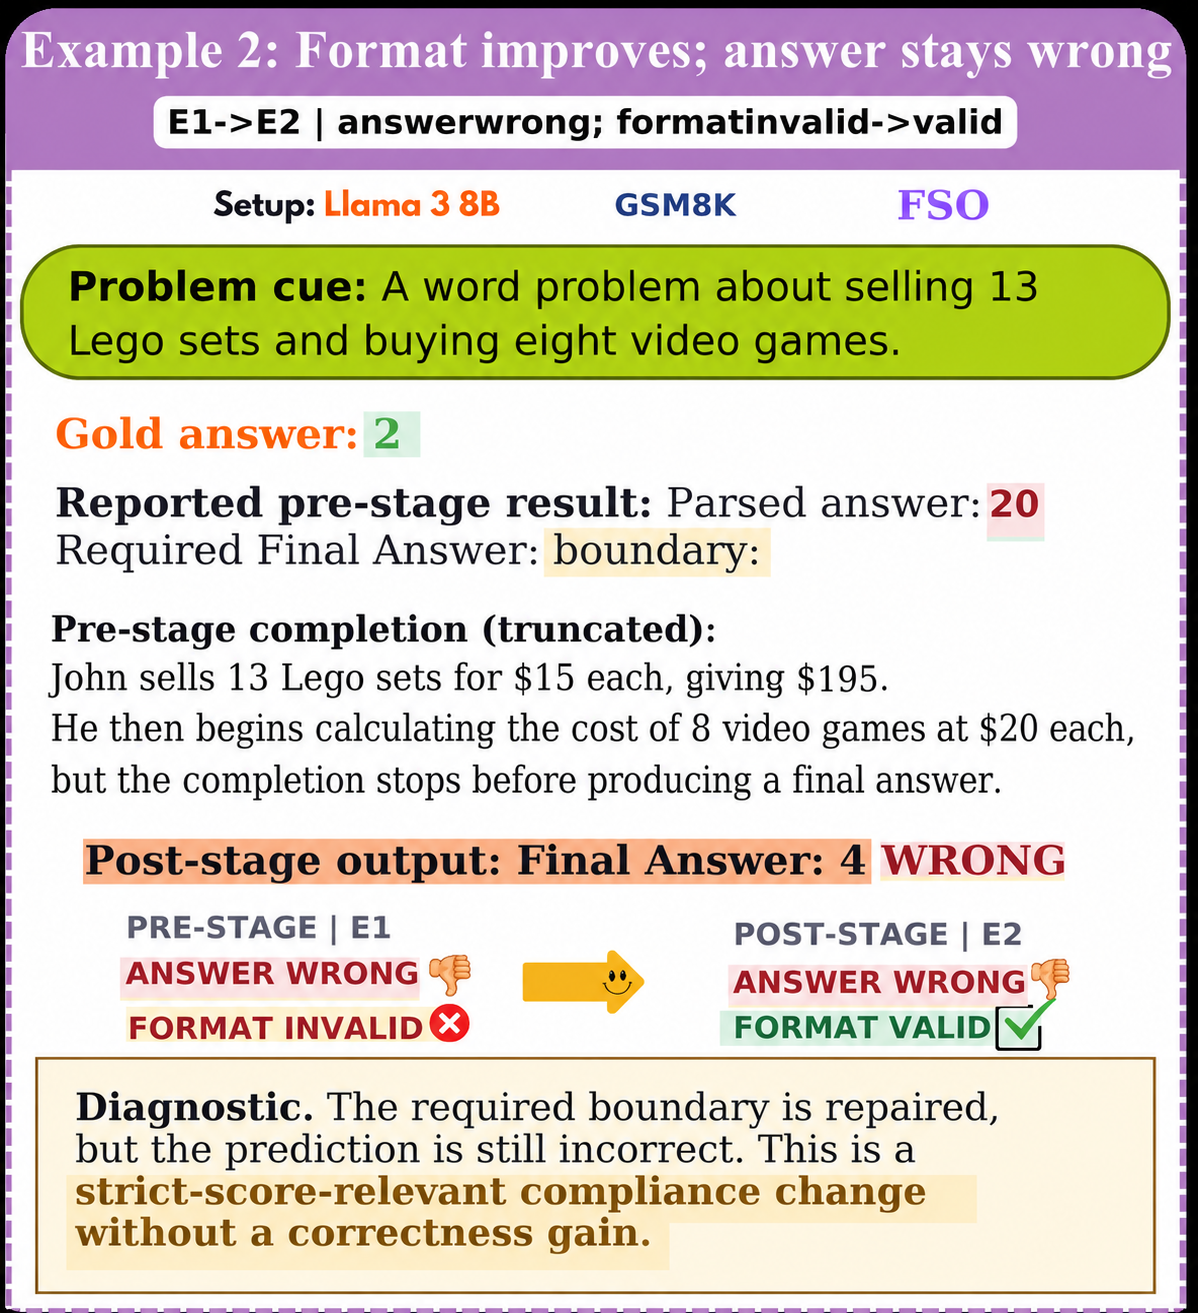
\includegraphics[width=0.485\linewidth,keepaspectratio]{Example_2.png}
\caption{\textbf{Compliance repairs.} Left: an already-correct StrategyQA response
becomes contract-valid ($\Ethree\!\to\!\Efour$), which raises the strict
score without any change in correctness. Right: a GSM8K response remains
incorrect while the required final-answer boundary is repaired
($\Eone\!\to\!\Etwo$), the single most common transition in the study.}
\label{fig:qualitative_format_examples}
\end{figure}

\begin{figure}[p]
\centering
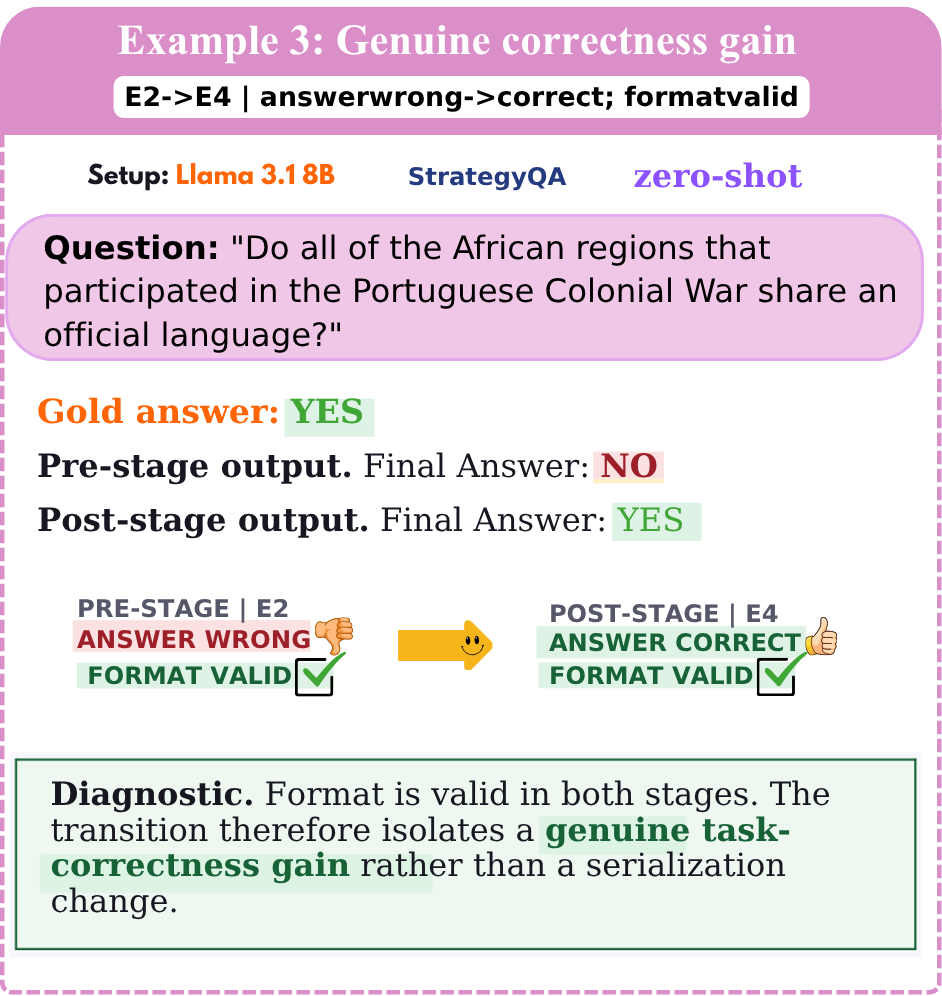
\includegraphics[width=0.485\linewidth,keepaspectratio]{Example_3.png}
\hfill
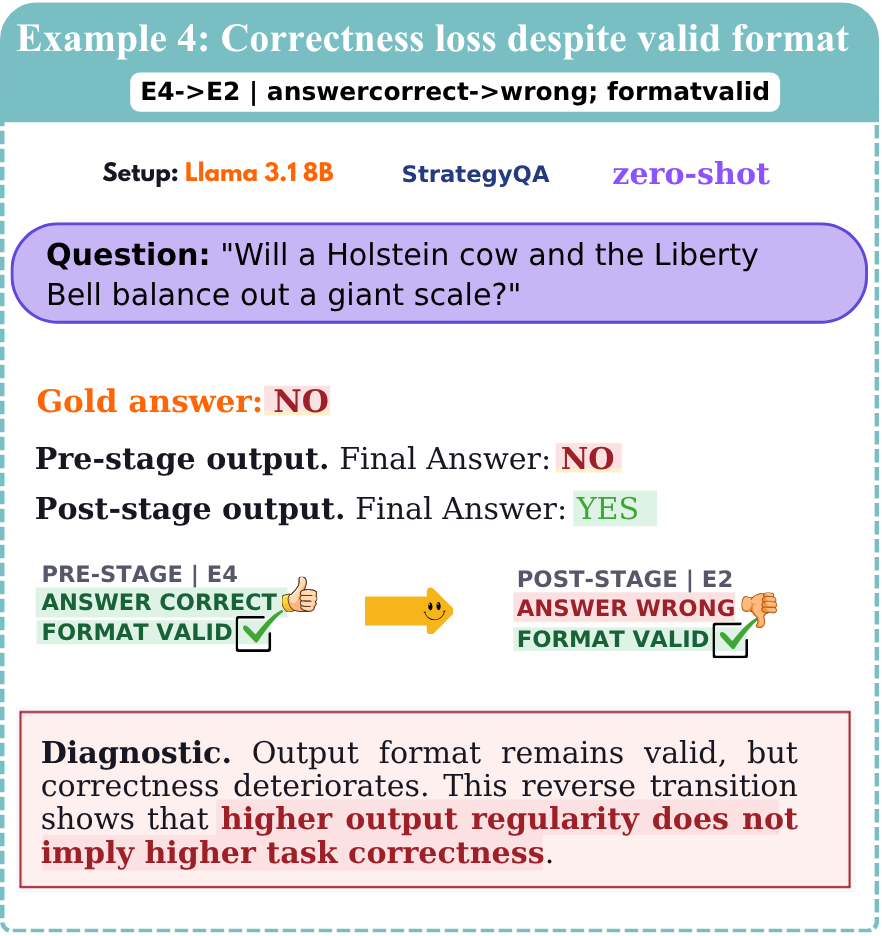
\includegraphics[width=0.485\linewidth,keepaspectratio]{Example_4.png}
\caption{\textbf{Correctness changes at constant compliance.} Left: incorrect to
correct while remaining format-valid ($\Etwo\!\to\!\Efour$). Right: correct
to incorrect while remaining format-valid ($\Efour\!\to\!\Etwo$). Improved
output regularity carries no information about which of these occurred.}
\label{fig:qualitative_correctness_examples}
\end{figure}

\begin{figure}[p]
\centering
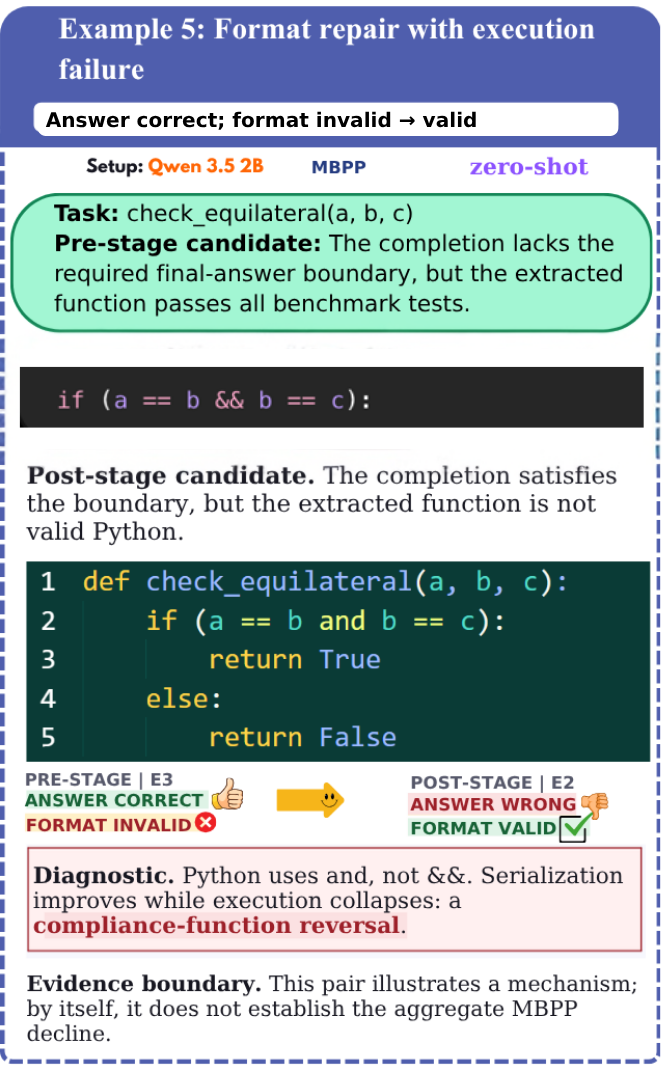
\includegraphics[width=0.485\linewidth,keepaspectratio]{Example_5.png}
\hfill
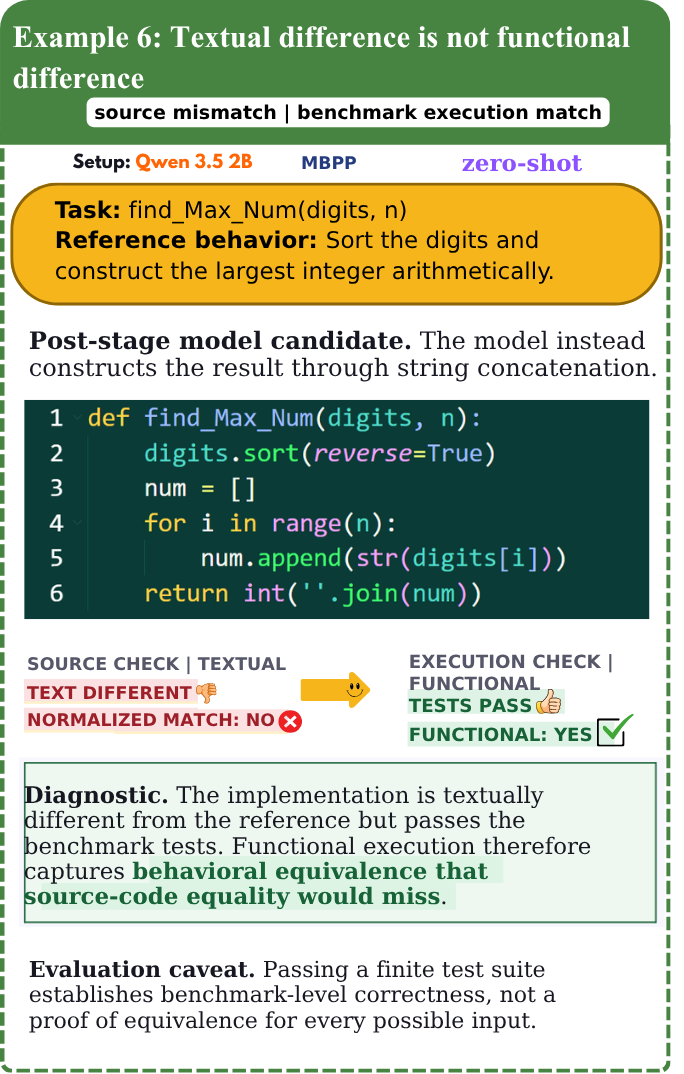
\includegraphics[width=0.485\linewidth,keepaspectratio]{Example_6.png}
\caption{\textbf{Execution-based MBPP examples.} Left: compliance improves while a
passing pre-SFT program is replaced by a boundary-compliant post-SFT program
that is not valid Python (\texttt{\&\&} in place of \texttt{and}), the
mechanism behind the syntax-error channel in Table~\ref{tab:mbpp_main}B.
Right: a generated implementation differs textually from the reference yet
passes the benchmark tests, illustrating why execution rather than source
agreement anchors programming claims. Passing a finite test suite establishes
benchmark-level correctness, not equivalence on every input.}
\label{fig:qualitative_mbpp_examples}
\end{figure}


\end{document}
